\documentclass[11pt]{article}
\RequirePackage{fullpage}
\RequirePackage[font=small,labelfont=bf]{caption}
\RequirePackage{amsmath,amssymb,amsthm}
\RequirePackage{graphicx}
\RequirePackage[hidelinks]{hyperref}
\RequirePackage{subcaption}
\RequirePackage{wasysym}
\RequirePackage{authblk}
\RequirePackage{bm}
\RequirePackage{bbm}
% \RequirePackage[osf]{mathpazo}
\RequirePackage[bibstyle=authoryear,citestyle=authoryear-comp,maxbibnames=9,maxcitenames=1,backend=biber,natbib=true,uniquelist=false,hyperref=true]{biblatex}
\usepackage{color}
\usepackage{nicefrac}

\renewcommand{\P}{\mathbb{P}}
\newcommand{\E}{\mathbb{E}}
\newcommand{\V}{\text{V}}
% \DeclareMathOperator{\var}{var}
% \DeclareMathOperator{\cov}{cov}

\newcommand{\msxa}{\mars_X}
\newcommand{\fsxa}{\venus_X}


\newcommand{\gc}[1]{{\it \color{red} #1 } }
\newcommand{\vb}[1]{{\it \color{blue} #1}}
\newtheorem{lemma}{Lemma}

\addbibresource{bib.bib}

\title{A Genealogical Look at Shared Ancestry on the X Chromosome}

\author[$\ast$,$1$]{Vince Buffalo}
\author[$\dag$]{Stephen M. Mount}
\author[$\ast$]{Graham Coop}
\affil[$\ast$]{\footnotesize Department of Evolution and Ecology, Center for Population Biology\protect\\University of California, Davis, CA 95616}
\affil[$\dag$]{\footnotesize Department of Cell Biology and Molecular Genetics, Center for Bioinformatics and Computational Biology\protect\\University of Maryland, College Park, MD 20742}
\affil[$1$]{\footnotesize Email for correspondence: vsbuffalo@ucdavis.edu}

\begin{document}

\maketitle
\thispagestyle{empty}

% **Data Policy**
% All of the code to reproduce all simulations for results and figures is
% freely available at this project's Github repository at
% https://github.com/vsbuffalo/x-ancestry. We have also included the raw
% simulation data here.

% **Keywords **
% X chromosome, genetic genealogy, statistical genetics, identity by descent, recent ancestry

% Article Summary
% Looking back through the generations, a person has two parents, four
% grandparents, eight great-grandparents, and so on. Due to the special
% inheritance pattern of the X chromosome, only a fraction of these ancestors can
% potentially share genetic material on the X chromosome with the present-day
% individual. We develop probabilistic models for how genetic material is shared
% between individuals in this X chromosome genealogy. Since homologous
% recombination on the X only occurs in females, and the number of females
% between a present-day individual and an X ancestor k generations back varies,
% genetic material survives at different rates across the X genealogy. Our models
% help in inferring details about recent ancestry beyond those possible with the
% autosomes alone.

\begin{abstract}
Close relatives can share large segments of their genome identical by descent
(IBD) that can be identified in genome-wide polymorphism datasets. There are a
range of methods to use these IBD segments to identify relatives and estimate
their relationship. These methods have focused on sharing on the autosomes, as
they provide a rich source of information about genealogical relationships. We
can hope to learn additional information about recent ancestry through shared
IBD segments on the X chromosome, but currently lack the theoretical framework
to use this information fully. Here, we fill this gap by developing probability
distributions for the number and length of X chromosome segments shared IBD
between an individual and an ancestor $k$ generations back, as well as between
half- and full-cousin relationships. Due to the inheritance pattern of the X
and the fact that X homologous recombination only occurs in females (outside of
the pseudo-autosomal regions), the number of females along a genealogical
lineage is a key quantity for understanding the number and length of the IBD
segments shared amongst relatives. When inferring relationships among
individuals, the number of female ancestors along a genealogical lineage will
often be unknown. Therefore, our IBD segment length and number distributions
marginalize over this unknown number of recombinational meioses through a
distribution of recombinational meioses we derive. We show how our results can
be used to estimate the number of female ancestors between two relatives,
giving us more genealogical details than possible with autosomal data alone.

\end{abstract}

{\small {\bf Keywords:} X chromosome, genetic genealogy, statistical genetics, identity by descent, recent ancestry}\\[1em]

Close relatives are expected to share large contiguous segments of their genome
due to the limited number of crossovers per chromosome each generation
\citep{fisher1949theory,fisher1954fuller,Donnelly:1983fi}. These large
identical by descent (IBD) segments shared among close relatives leave a
conspicuous footprint in population genomic data, and identifying and
understanding this sharing is key to many applications in biology
\citep{thompson2013identity}. For example, in human genetics, evidence of
recent shared ancestry is an integral part of detecting cryptic relatedness in
genome-wide association studies \citep{gusev2009whole}, discovering
mis-specified relationships in pedigrees \citep{sun2002enhanced}, inferring
pairwise relationships \citep{Epstein:2000b, glaubitz2003prospects,
huff2011maximum}, and localizing disease traits in pedigrees
\citep{thomas2008shared}. In forensics, recent ancestry is crucial for both
accounting for population-level relatedness \citep{balding1994dna} and in
familial DNA database searches \citep{belin1997summarizing,
sjerps1999consequences}. Additionally, recent ancestry detection methods have a
range of applications in anthropology and ancient DNA to understand the
familial relationships among sets of individuals
\citep{Fu:2015bl,keyser2003nuclear,baca2012ancient,haak2008ancient}. In
population genomics, recent ancestry has been used to learn about recent
migrations and other demographic events
\citep{ralphcoop2013,palamara2012length}. An understanding of recent ancestry
also plays a large role in understanding recently admixed populations, where
individuals draw ancestry from multiple distinct populations
\citep{pool2009inference,Gravel:2012ip,Liang:2014fo}. Finally, relative finding
through recent ancestry is increasingly a key feature of direct-to-consumer
personal genomics products and an important source of information for
genealogists leveraging genetic information
\citep{Durand010512,royal2010inferring}. 

Approaches to infer recent ancestry among humans have often used only the
autosomes, as the recombining autosomes offer more opportunity to detect a
range of relationships than the Y chromosome, mitochondria, or X chromosome.
However, the nature of X chromosome inheritance means that it can clarify
details of the relationships among individuals and be informative about
sex-specific demography and admixture histories in ways that autosomes cannot
\citep{Goldberg:2015ja,ramachandran2004robustness,
ramachandran2008population,bryc2010genome,Bustamante:2009gp,Shringarpure039347,pool2007population}.

In this paper, we look at the inheritance of chromosomal segments on the X
chromosome among closely related individuals. Our genetic ancestry models are
structured around biparental genealogies back in time, an approach used by many
previous authors \citep[e.g.,][]{Donnelly:1983fi,
chang1999recent,Barton:2011iq,Rohde:2004kl}. If we ignore pedigree collapse
(due to inbreeding), the genealogy of a present-day individual encodes all
biparental relationships back in time; e.g. the two parents, four grandparents,
eight great-grandparents, $2^k$ $\text{great}^{k-2}$ grandparents, and in
general the $2^k$ ancestors $k$ generations back; we refer to these individuals
as one's \emph{genealogical ancestors}. Note that throughout this paper,
\emph{ancestors} refers to the ancestors within generation $k$, not the total
number of ancestors from generations 1 to $k$, $\sum_{i=1}^k 2^i$. A
genealogical ancestor of a present-day individual is said to also be a
\emph{genetic ancestor} if the present-day individual shares genetic material
by descent from this ancestor.  We refer to these segments of shared genetic
material as being identical by descent, and in doing so we ignore the
possibility of mutation in the limited number of generations separating our
individuals. Throughout this paper, we will ignore the pseudo-autosomal (PAR)
region of the X chromosome, which undergoes crossing over with the Y chromosome
in males \citep{koller1934genetical} to ensure proper disjunction in meiosis I
\citep{hassold1991xy}. We also ignore gene conversion which is known to occur
on the X \citep{Rosser:2009df}. 

Here, we are concerned with inheritance through the \emph{X genealogy} embedded
inside an individual's genealogy, which includes only the subset of one's
genealogical ancestors who could possibly contributed to one's non-PAR X
chromosome. We refer to the individuals in this X genealogy as \emph{X
ancestors}. Since males receive an X only from their mothers, a male's father
cannot be an X ancestor. Consequently, a male's father and all of his ancestors
are excluded from the X genealogy (Figure \ref{fig:x-rm-tree}). Therefore,
females are overrepresented in the X genealogy, and as we go back in one's
genealogy, the fraction of individuals who are possible X ancestors shrink.
This property means that genetic relationships differ on the X compared to the
autosomes, a fact that changes the calculation of kinship coefficients on the X
\citep{pinto2012general,pinto2011x} and also has interesting implications for
kin-selection models involving the X chromosome
\citep{Fox:2009kh,rice2008sexually}.

\begin{figure}[!ht]
  \centering
  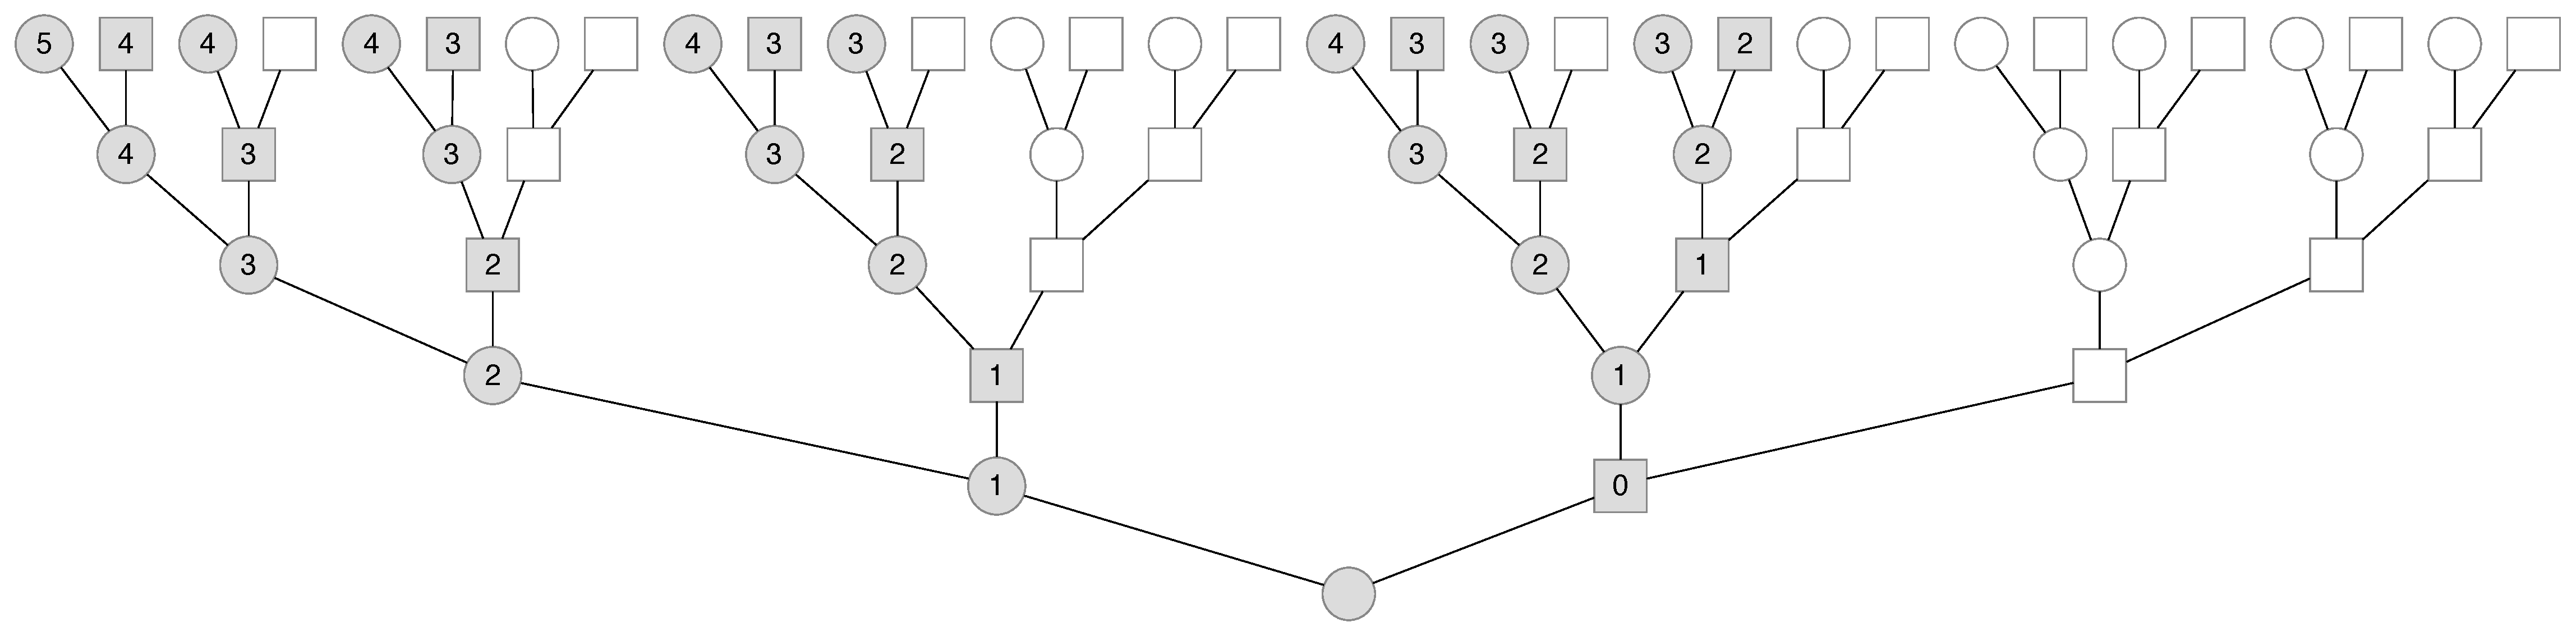
\includegraphics[width=\textwidth]{images/x-rm-tree.eps}

  \caption{An example genealogy with the embedded X genealogy back five
    generations. Males are depicted as squares and females as circles.
    Individuals in the X genealogy are shaded gray while unshaded individuals
    are ancestors that are not X ancestors. Each X ancestor is labeled with the
  number of recombinational meioses to the present-day female.}
  \label{fig:x-rm-tree}
\end{figure}

In Section \ref{sec:auto-ancestry} we review models of autosomal identity by
descent among relatives, on which we base our models of X genetic ancestry.
Then, in Section \ref{sec:x-ancestry} we look at X genealogies back in time, as
the properties of X genealogies affect the transmission of X genetic material
from X ancestors to a present-day individual. We develop simple approximations
to the probability distributions of the number and length of X chromosome
segments that will be shared IBD between a present-day female and one of her X
ancestors a known number of generations back in time. These models provide a
set of results for the X chromosome equivalent to those already known for the
autosomes \citep{Donnelly:1983fi,thomas:1994hg}. Then, in Section
\ref{sec:shared-x-anc}, we look at shared X ancestry---when two present-day
cousins share an X ancestor a known number of generations back. We calculate
the probabilities that genealogical half- and full-cousins are also connected
through their X genealogy, and thus can potentially share genetic material on
their X. We then extend our models of IBD segment length and number to segments
shared between half- and full-cousins. Finally, in Section \ref{sec:inf} we
show that shared X genetic ancestry contains additional information (compared
to genetic autosomal ancestry) for inferring relationships among individuals,
and explore the limits of this information. 

\section{Autosomal Ancestry}
\label{sec:auto-ancestry}

To facilitate comparison with our X chromosome results, we first briefly review
analogous autosomal segment number and segment length distributions
\citep{Donnelly:1983fi,thomas:1994hg,huff2011maximum}. Throughout this paper,
we assume that one's genealogical ancestors $k$ generations back are distinct,
i.e. there is no pedigree collapse due to inbreeding (see Appendix
\ref{ap:ped-collapse} for a model of how this assumption breaks down with
increasing $k$). Thus, an individual has $2^k$ \emph{distinct} genealogical
ancestors. Assuming no selection and fair meiosis, a present-day individual's
autosomal genetic material is spread across these $2^k$ ancestors with equal
probability, having been transmitted to the present-day individual solely
through recombination and fair segregation.

We model the process of crossing over during meiosis as a continuous time
Markov process along the chromosome, as in \textcite{thomas:1994hg} and
\textcite{huff2011maximum}, and described by \textcite{Donnelly:1983fi}. In
doing so we assume no crossover interference, such that in each generation $b$
recombinational breakpoints occur as a Poisson process running with a uniform
rate equal to the total length of the genetic map (in Morgans), $\nu$. Within a
single chromosome, $b$ breaks creates a mosaic of $b+1$ alternating pieces of
maternal and paternal segments. This alternation between maternal and paternal
haplotypes creates long-run dependency between segments. We ignore these
dependencies in our analytic models by assuming that each chromosomal segment
survives segregation independently with probability \nicefrac{1}{2} per
generation. For $d$ independent meioses separating two individuals, we imagine
the Poisson recombination process running at rate $\nu d$, and for a segment to
be shared IBD between the two ancestors it must survive $\nicefrac{1}{2^d}$
segregations.  Consequently, the expected number of segments shared IBD between
two individuals $d$ meioses apart in a genome with $c$ chromosomes is
approximated as \citep{thomas:1994hg}:

\begin{align}
  \label{eq:exp-n}
  \E[N] &= \frac{1}{2^d} (\nu d + c)
\end{align}

Intuitively, we can understand the $\nicefrac{1}{2^d}$ factor as the
coefficient of kinship \citep[or path
coefficient;][]{wright1922coefficients,wright1934method} of two individuals $d$
meioses apart, which gives the probability that two alleles are shared IBD
between these two individuals. Then, the expected number of IBD segments
$\E[N]$ can be thought of as the average number of alleles shared between two
individuals in a genome with $\nu d + c$ loci total. Under this approximation,
recombination increases the number of independent loci linearly each generation
(by a factor of the total genetic length). A fraction $\nicefrac{1}{2^d}$ of
parental alleles at these loci survive the $d$ meioses to be IBD with the
present-day individual.

By convention, we count the number of contiguous IBD segments $N$ in the
present-day individual, not the number of contiguous segments in the ancestor.
For example, an individual will share exactly one block per chromosome with
each parent if we count the contiguous segments in the offspring, even though
these segments may be spread across the parent's two homologues. This
convention, which we use throughout the paper, is identical to counting the
number of IBD segments that occur in $d-1$ meioses rather than $d$ meioses.
This convention only impacts models of segments shared IBD between an
individual and one of their ancestors; neither the distribution of segment
lengths nor the distributions for segment number shared IBD between cousins are
affected by this convention.

\paragraph{The distribution of IBD segments between a present-day individual
and an ancestor} 
\label{sec:auto-dist-ibd-seg}

Given that a present-day individual and an ancestor in the $k^\text{th}$
generation are separated by $k$ meioses, the number of IBD segments can be
modeled with what we call the \emph{Poisson-Binomial} approximation. Over $d=k$
meioses, $B=b \sim \text{Pois}(\nu k)$ recombinational breakpoints fall on $c$
independently assorting chromosomes, creating $b + c$ segments. Ignoring
long-range dependencies, we assume all of these $b+c$ segments have an
independent chance of surviving the $k$ segregations to the present-day
individual, and thus the probability that $n$ segments survive given $b+c$
trials is Binomially distributed with probability $\nicefrac{1}{2^k}$.
Marginalizing over the unobserved number of recombinational breakpoints $b$,
and replacing $k$ with $k-1$ to following the convention described above:

\begin{equation}
  P(N=n | k) = \sum_{b=0}^\infty \text{Bin}(N=n \;|\; l=b+c,
p=\nicefrac{1}{2^{k-1}}) \; \text{Pois}(B=b \;|\; \lambda=\nu (k-1))
\end{equation}

The expected value of the Poisson-Binomial model is given by equation
\eqref{eq:exp-n} with $d=k-1$ and this model is similar to those of
\textcite{thomas:1994hg,Donnelly:1983fi}. We can further approximate this by
assuming that we have a Poisson total number of segments with mean $(c +
\nu(k-1))$ and these segments are shared with probability
$\nicefrac{1}{2^{k-1}}$ as in \textcite{huff2011maximum}. This gives us a
thinned Poisson distribution of shared segments:

\begin{align}
\label{eq:auto-segment-number}
  P(N = n | k, \nu, c) &= \text{Pois}(N = n | \lambda = (c + \nu (k-1))/2^{k-1}) \nonumber \\
                       &= \frac{((c + \nu (k-1))/2^{k-1})^n  e^{- (c + \nu (k-1))/{2^{k - 1}}}}{n!}
\end{align}

This thinned Poisson model also has an expectation given by equation
\eqref{eq:exp-n} but compared to the Poisson-Binomial model has a larger
variance than the true process. This overdispersion occurs because modeling the
number of segments created after $b$ breakpoints involves incorporating the
initial number of chromosomes into the Poisson rate. However, this initial
number of chromosomes is actually fixed, which the Poisson-Binomial model
captures but the Poisson thinning model does not (i.e. one generation back such
that $k=1$, the thinning model treats the number of segments shared IBD with
one's parents is $N \sim \text{Pois}(c)$ rather than $c$). See Appendix
\ref{ap:pois-thin} for a further comparison of these two models. A more formal
description of this approximation as a continuous-time Markov process is given
in \textcite{thomas:1994hg}.

\paragraph{The distribution of IBD segments between cousins}

Similarly, we can derive the distribution for the number of IBD segments shared
between two half-cousins with an ancestor in the $k^\text{th}$ generation. Two
half-cousins are separated by $2k$ meioses, thus the distribution for number of
segments is:

\begin{equation} \label{eq:auto-seg-cousins}
 P(N=n \;|\; k, \nu, c) = \text{Pois}\left(N = n \;|\; \lambda=(c + 2 k \nu)/2^{2 k - 1} \right)
\end{equation}
%
Since either of the shared ancestor's haplotypes can be shared IBD between the
two cousins, the Poisson process rate is doubled. Full-cousins can share segments
via either of their two shared ancestors, leading the distribution to be:

\begin{equation}
  P(N=n \;|\; k, \nu, c) = \text{Pois}\left(N = n \;|\; \lambda=(c + 2 k \nu)/2^{2 k - 2} \right)
\end{equation}


\paragraph{The distribution of autosome segment lengths}

In addition to the number of IBD segments, the length of segments is also
informative about ancestry \citep[e.g.][]{palamara2012length}. As we model
crossing over as a Poisson process, a one Morgan region will experience on
average $d$ recombination events over $d$ meioses. Therefore, the probability
density of segment lengths shared IBD between two individuals $d$ meioses apart
is exponential with rate $d$:

\begin{equation}
  \label{eq:auto-seg-lens}
  p(U=u | d) = d e^{-du}
\end{equation}

Equations \eqref{eq:auto-seg-lens} and \eqref{eq:auto-seg-cousins} specify a
model of the number and lengths of segments shared between various degree
relatives. Various authors have used these types of results to derive
likelihood-based models for classifying the genealogical relationship between
pairs of individuals using autosome IBD data
\citep{huff2011maximum,Henn:2012ij,Durand010512}. 

We will use similar models as these in modeling the length and number of X
chromosome segments shared been relatives. However, the nature of X genealogies
(which we cover in the next section) requires we adjust these models.
Specifically, while one always has $k$ recombinational meioses between an
autosomal ancestor in the $k^\text{th}$ generation, the number of
recombinational meioses varies across the lineages to an X ancestor with the
number of females in a lineage, since X homologous recombination only occurs in
females (Figure \ref{fig:x-rm-tree}). This varying number of recombinational
meioses across lineages leads to a varying-rate Poisson recombination process,
with the rate depending on the specific lineage to the X ancestor. After we
take a closer look at X genealogies in the next section, we adapt the models
above to handle the varying-rate Poisson process needed to model IBD segments
in X genealogies.

\begin{figure}[!ht]
    \centering
    % change 0.49 to 0.5 for vertical alignment of subfigures
    \begin{subfigure}[b]{0.8\textwidth}
      % 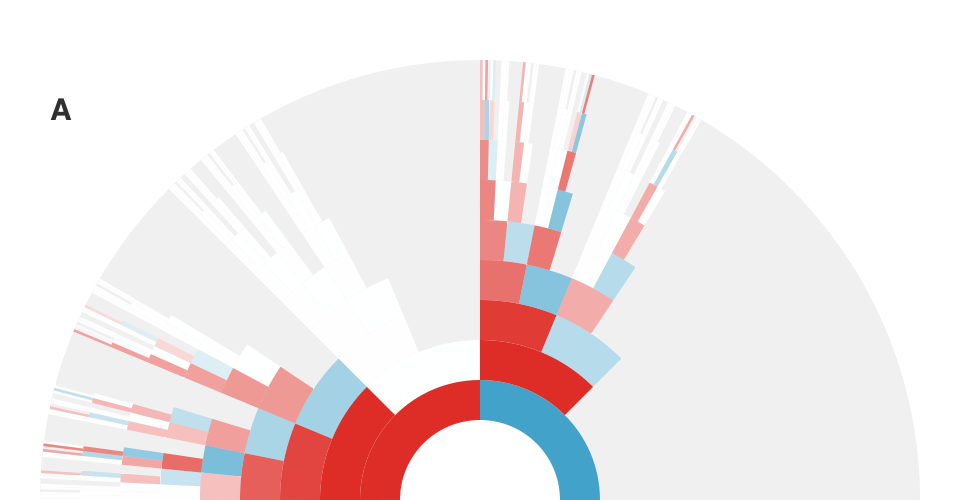
\includegraphics[width=\textwidth]{images/x-arc.png}
      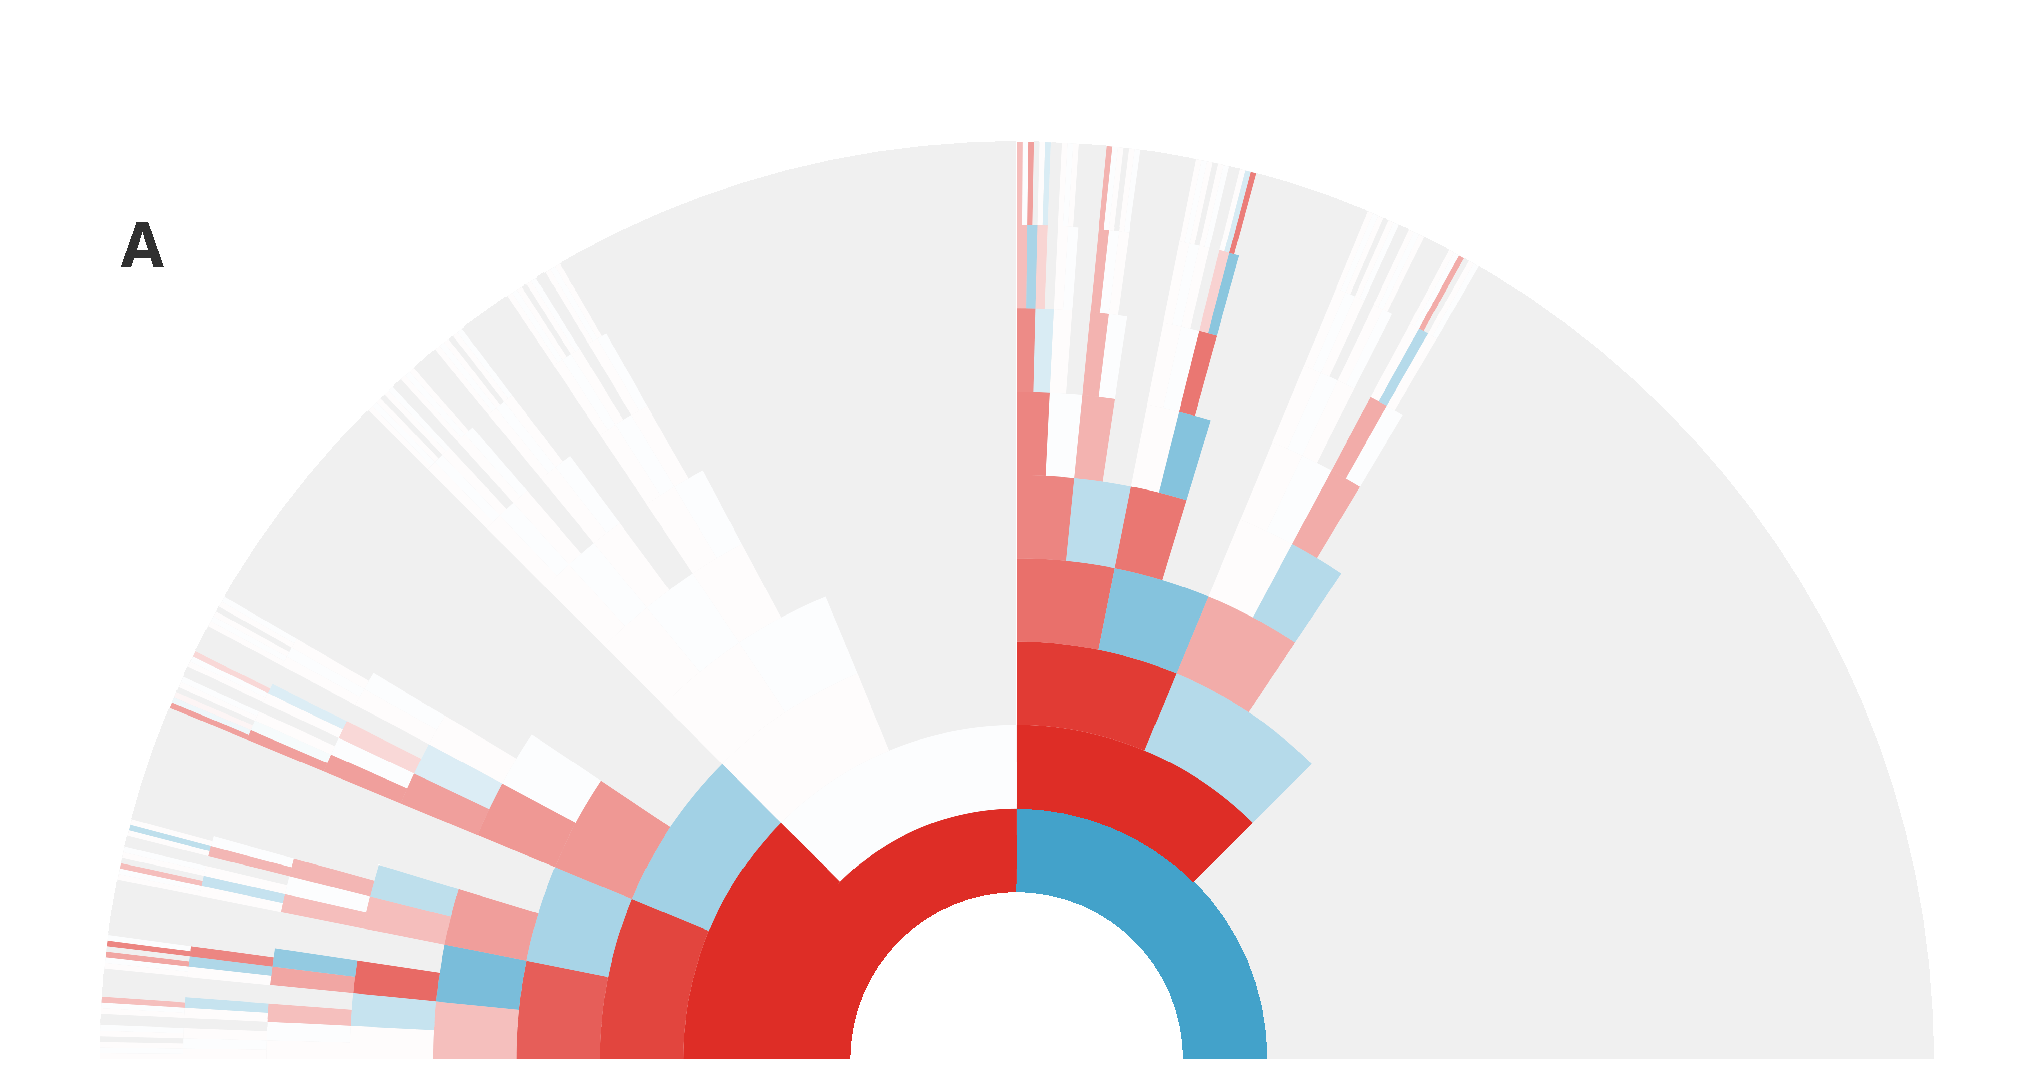
\includegraphics[width=\textwidth]{images/x-arc}
    \end{subfigure}
    \begin{subfigure}[b]{0.8\textwidth}
      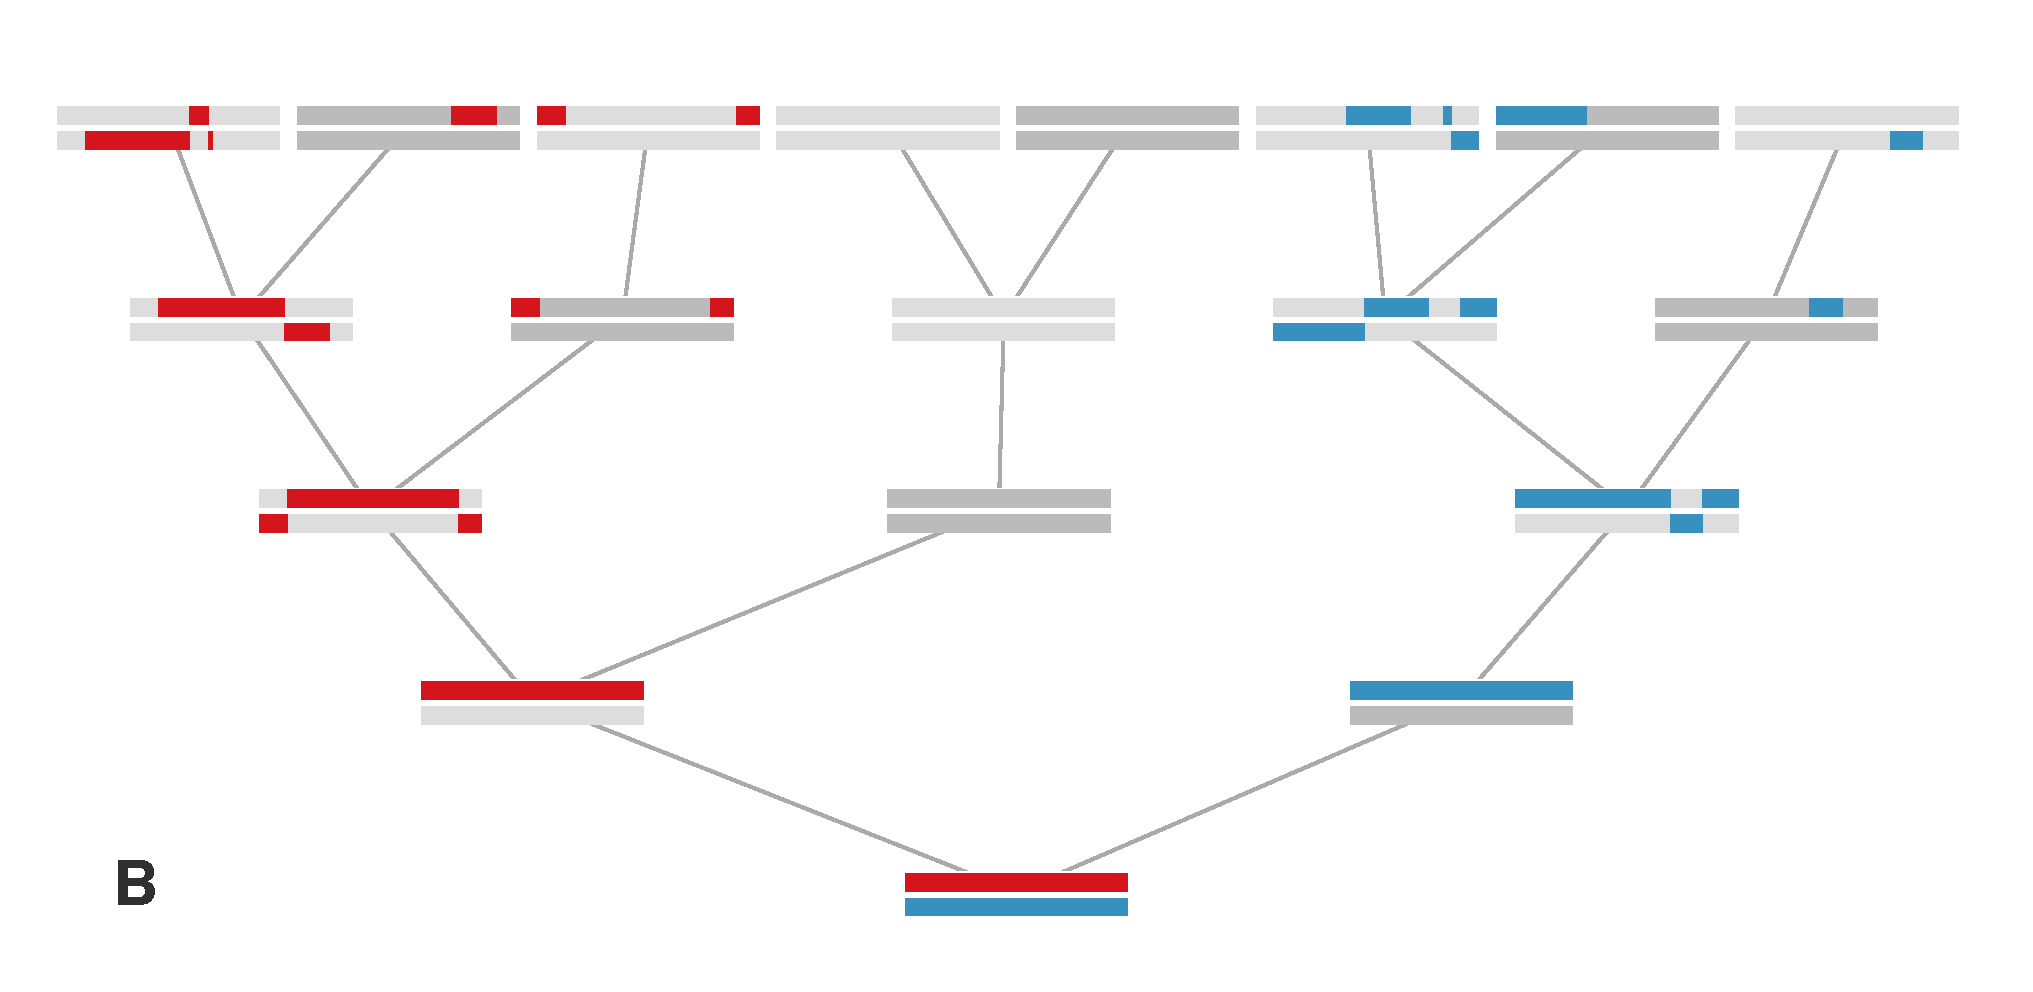
\includegraphics[width=\textwidth]{images/x-tree}
    \end{subfigure}
    
    \caption{A: Simulated X genealogy of a present-day female, back nine
      generations.  Each arc is an ancestor, with female ancestors colored red,
      and male ancestors colored blue. The transparency of each arc reflects
      the genetic contribution of this ancestor to the present-day female.
      White arcs correspond to an X genealogical ancestor that shares no
      genetic material with the present-day female, and gray arcs are
      genealogical ancestors that are not X ancestors. B: The X segments of the
      simulation in (A), back five generations.  The maternal X lineage's
      segments are colored red, and the paternal X segments are colored blue. A
      male ancestor's sex chromosomes are colored dark gray (and include the Y)
    and a female ancestor's sex chromosomes are colored light gray.}

    \label{fig:x-arc}

  \end{figure}


\section{X Ancestry}
\label{sec:x-ancestry}

\paragraph{Number of Genealogical X Ancestors}

  \begin{figure}[!ht]
    \centering
    % change 0.49 to 0.5 for vertical alignment of subfigures
    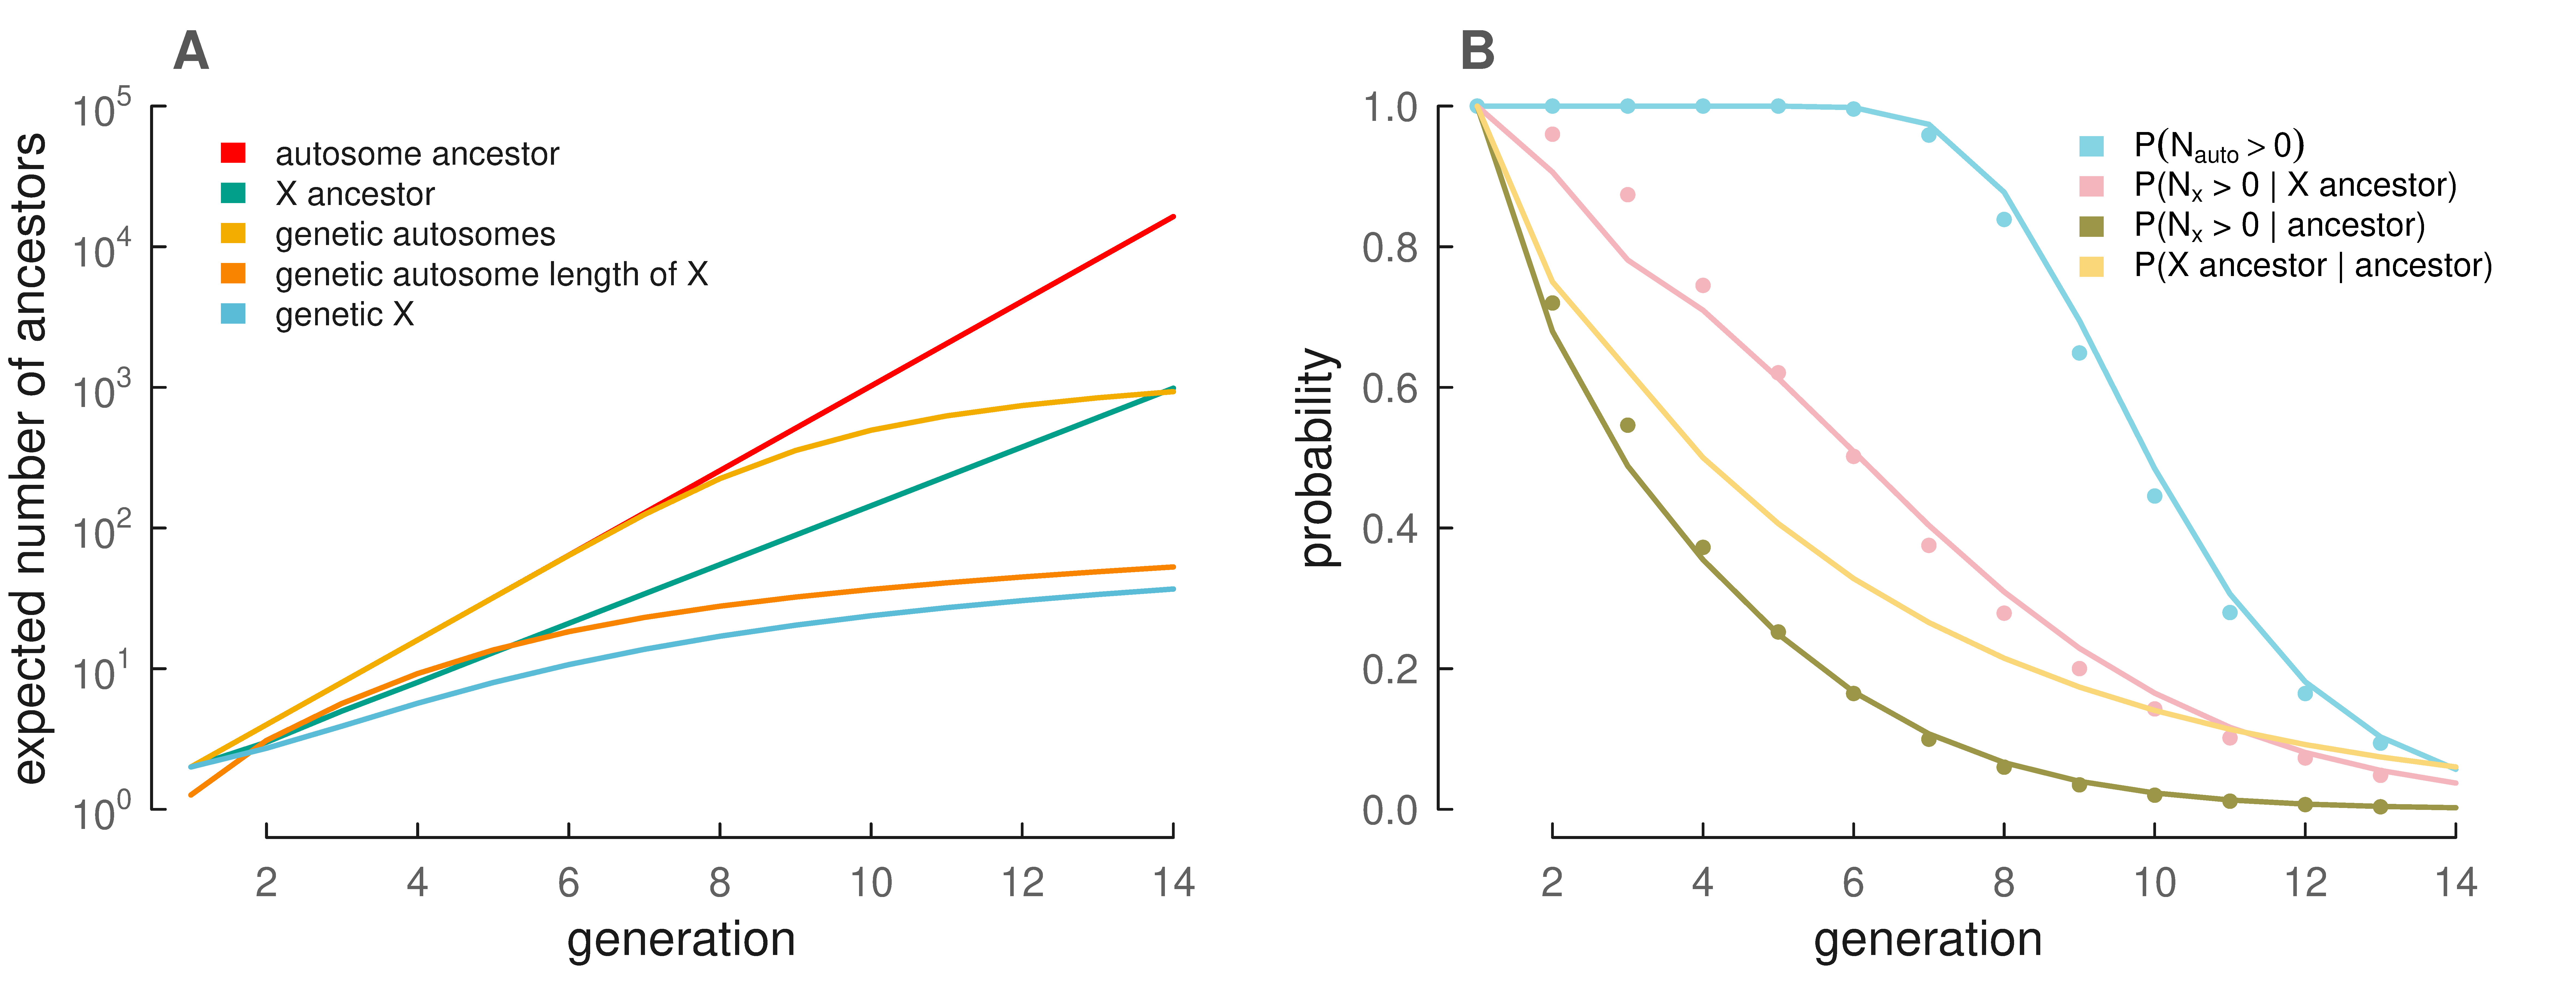
\includegraphics[width=\textwidth]{images/num-ancestors}

    \caption{A: Each line represents a present-day female's number ancestors
(y-axis) in the $k^\text{th}$ generation (x-axis; where $k=1$ is parental
generation), for a variety of cases. The present day's number of genealogical
ancestors in the $k^\text{th}$ generation is in red, and the expected number of
these ancestors that contribute any autosome genetic material is in yellow.
Likewise, the present-day female's genealogical X ancestors is in green, and
the expected number of these ancestors that contribute any X genetic material
is in blue. For comparison, the number of genetic ancestors of an autosome of
length equal to the X is included (orange).  B: The probability of genealogical
and genetic ancestry (y-axis) from an arbitrary ancestor in the $k^\text{th}$
generation (x-axis). $P(\text{N}_\text{auto} > 0)$ is derived from equation
\eqref{eq:auto-segment-number}, $P(\text{N}_\text{X} > 0 \;|\; \text{X
ancestor})$ from equation \eqref{eq:x-number-block}, $P(\text{N}_\text{X} > 0
\;|\; \text{ancestor})$ from equations \eqref{eq:x-number-block} and
\eqref{eq:prob-x-anc}, and $P(\text{X ancestor} \;|\; \text{ancestor})$ from
equation \eqref{eq:prob-x-anc}. Points show simulated results.}

\label{fig:num-ancestors}
\end{figure}

While a present-day individual can potentially inherit autosomal segments from
any of its $2^k$ genealogical ancestors $k$ generations back, only a fraction
of these individuals can possibly share segments on the X chromosome. In
contrast to biparental genealogies, males have only one genealogical X
ancestor---their mothers---if we ignore the PAR. This constraint (which we
refer to throughout as the \emph{no two adjacent males condition}) shapes both
the number of X ancestors and the number of females along an X lineage. For
example, consider a present-day female's X ancestors one generation back: both
her father and mother contribute X chromosome material. Two generations back,
she has three X genealogical ancestors: her father only inherits an X from her
paternal grandmother, while her mother can inherit X material from either of
parents. Continuing this process, this individual has five X ancestors three
generations back and eight ancestors four generations back (Figure
\ref{fig:x-rm-tree}). 


In general, a present-day female's X genealogical ancestors is growing as a
Fibonacci series \citep{laughlin1920calculating, Basin:1963wf}, such that $k$
generations back she has $\mathcal{F}_{k+2}$ X genealogical ancestors, where
$\mathcal{F}_k$ is the $k^\text{th}$ Fibonacci number (where $k$ is 0-indexed
and the series begins $F_0 = 0, F_1 = 1, \ldots$; Online Encyclopedia of
Integer Sequences reference \href{https://oeis.org/A000045}{A000045};
\citeauthor{sloane2014online}, \citeyear{sloane2014online}). We can demonstrate
that one's number of X genealogical ancestors ($n_k$) grows as a Fibonacci
series by encoding the X inheritance rules for the number of males and females
($m_k$ and $f_k$, respectively) in the $k^\text{th}$ generation as a set of
recurrence relations:

\begin{align*}
  f_k &= n_{k-1} && \text{every individual receives an X chromosome from his/her mother}\\
  m_k &= f_{k-1} && \text{every female receives an X chromosome from her father}\\
  n_k &= f_k + m_k
\end{align*}

Rearranging these recurrence equations gives us $n_k = n_{k-1} + n_{k-2}$,
which is the Fibonacci recurrence. Starting with a female in the $k=0$
generation, we have initial values $n_0=1$ and $n_1 = 2$, which gives us the
Fibonacci numbers offset by two, $\mathcal{F}_{k+2}$. For a present-day male,
his number of X ancestors is $\mathcal{F}_{k+1}$, i.e. offset by one to count
the number of X ancestors his mother has. To simplify our expressions, we will
assume throughout the paper that all-present day individuals are female since a
simple offset can be made to handle males.

%\paragraph{Proportion of X ancestors} 


In Figure \ref{fig:num-ancestors}A we show the increase in the number of X
genealogical and genetic ancestors and compare these to the growth of all of
one's genealogical ancestors and autosomal genetic ancestors. The closed-form
solution for the $k^\text{th}$ Fibonacci number is given by Binet's formula,
which shows that the Fibonacci sequence grows at an exponential rate slower
than $2^k$. 

Consequently, the fraction of ancestors who can contribute to the X chromosome
declines with $k$. Given that a female has $\mathcal{F}_{k+2}$ X ancestors and
$2^k$ genealogical distinct ancestors, her proportion of X ancestors is:

\begin{equation}
  \label{eq:prob-x-anc}
  P(\text{X ancestor} \;|\; \text{ancestor}) = \frac{\mathcal{F}_{k+2}}{2^k} 
\end{equation}
%
This fraction can also be interpreted as the probability that a randomly chosen
genealogical ancestor $k$ generations ago is also an X genealogical ancestor.
We show this probability as a function of generations into the past in Figure
\ref{fig:num-ancestors}B (yellow line).

From our recurrence equations we can see that a present-day female's
$\mathcal{F}_{k+2}$ ancestors in the $k^\text{th}$ generation are composed of
$\mathcal{F}_{k+1}$ females and $\mathcal{F}_{k}$ males. Likewise for a
present-day male, his $\mathcal{F}_{k+1}$ ancestors in the $k^\text{th}$
generation are composed of $\mathcal{F}_{k}$ females and $\mathcal{F}_{k-1}$
males. We will use these results when calculating the probability of a shared X
ancestor.

\paragraph{Ancestry Simulations} 

In the next sections, we use stochastic simulations to verify the analytic
approximations we derive; here we briefly describe the simulation methods. We
have written a C and Python X genealogy simulation procedure (source code
  available in the supplement and at
\url{https://github.com/vsbuffalo/x-ancestry/}). We simulate a female's X
chromosome genetic ancestry back through her X genealogy. Each simulation
begins with two present-day female X chromosomes, one of which is passed to her
mother and one to her father. Segments transmitted to a male ancestor are
simply passed directly back to his mother (without recombination). For segments
passed to a female ancestor, we place a Poisson number of recombination
breakpoints (with mean $\nu$) on the X chromosome and the segment is broken
where it overlaps these recombination events. The first segment along the
chromosome is randomly drawn to have been inherited from either her
mother/father, and we alternate this choice for subsequent segments. This
procedure repeats until the target generation back $k$ is reached. The segments
in the $k$-generation ancestors are then summarized as either counts (number of
IBD segments per individual) or lengths.  These simulations are necessarily
approximate as they ignore crossover interference.  However, unlike our
analytic approximations, our simulation procedure maintains long-run
dependencies created during recombination, allowing us to see the extent to
which assuming independent segment survival adversely impacts our analytic
results.

Figure \ref{fig:x-arc}A depicts the X genetic ancestors of one simulated
example X genealogy back nine generations to illustrate this process. Each arc
represents a single ancestor of a present-day female; red arcs are female X
ancestors and blue arcs are male X ancestors. Ancestors that are not X
ancestors are shaded gray. The saturation indicates the genetic contribution of
this individual to the present-day female's X (with white indicating an X
ancestor that made no genetic contribution on the X). Figure \ref{fig:x-arc}B
shows the underlying X chromosome IBD segments for this same simulation back
four generations.

\paragraph{The number of recombinational meioses along an unknown X lineage}

If we pick an ancestor at random $k$ generations ago, the probability that they
are an X genealogical ancestor is given by equation \eqref{eq:prob-x-anc}. We
can now extend this logic and ask: having randomly sampled an X genealogical
ancestor, how many recombinational meioses (i.e. females) lie in the lineage
between a present day individual and this ancestor? Since IBD segment number
and length distributions are parameterized by a rate proportional to the number
of recombination events, this quantity is essential to our further derivations.

\begin{figure}[!ht]
  \centering
  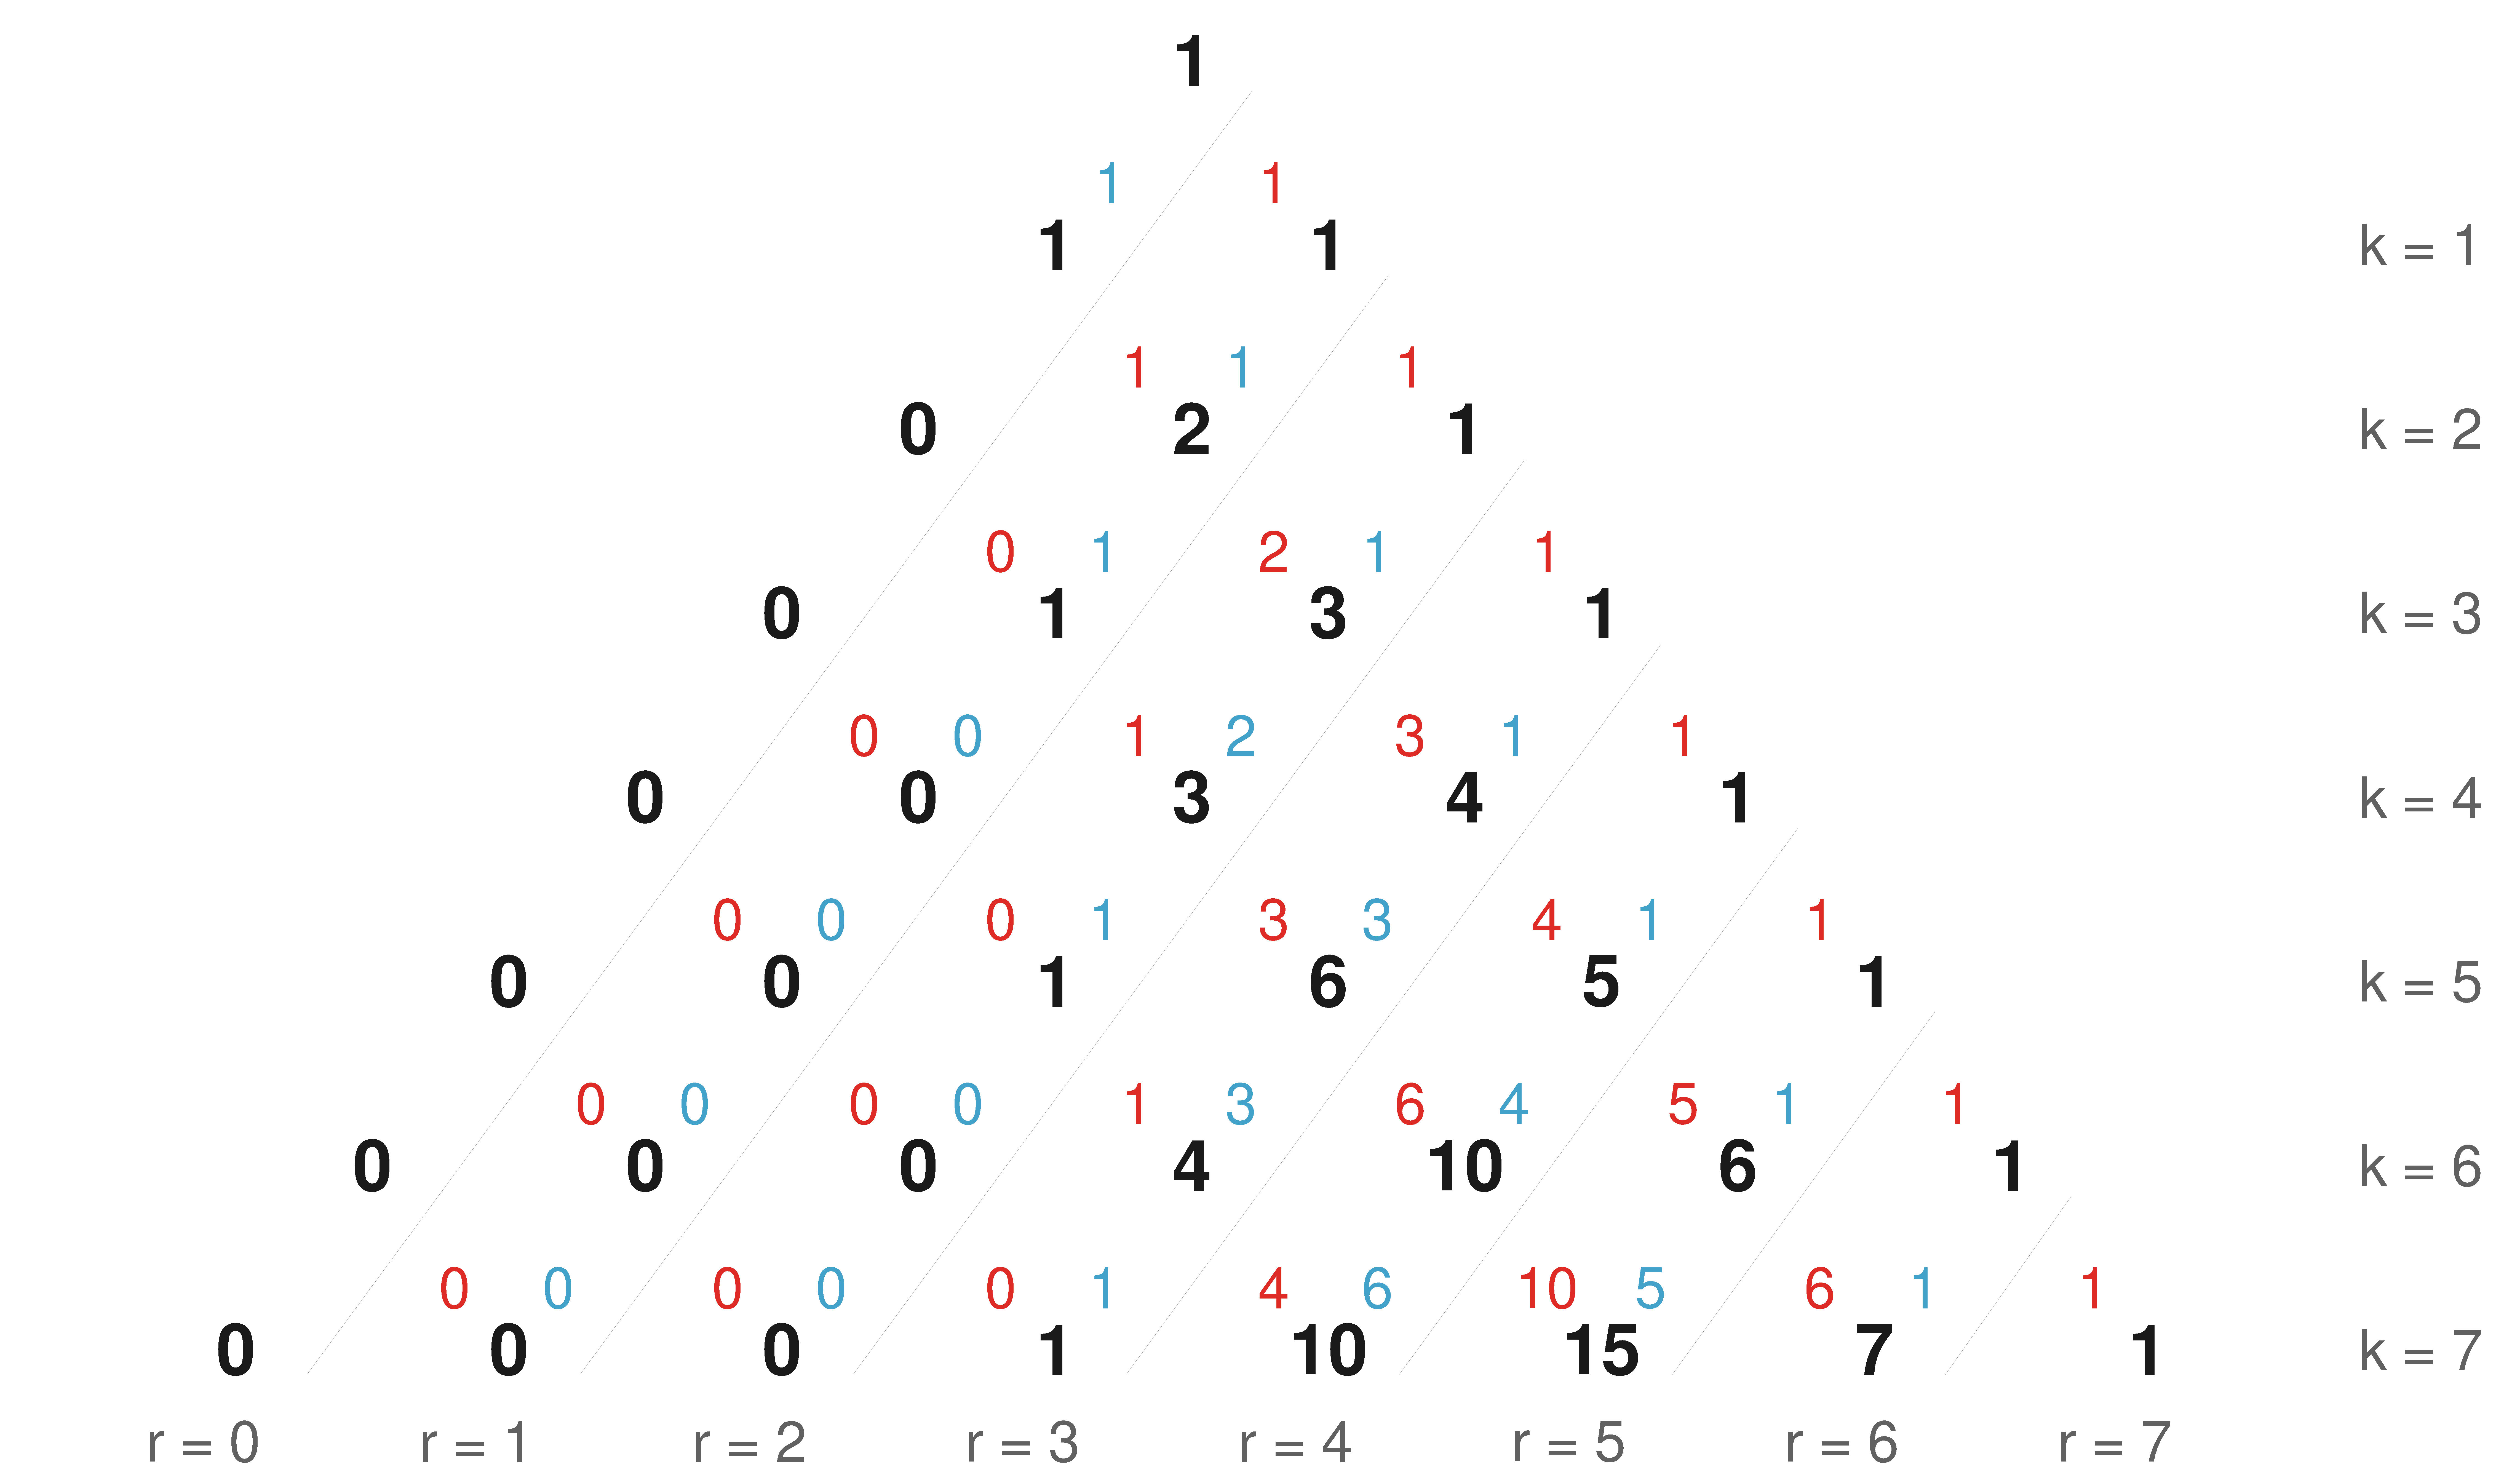
\includegraphics[width=0.7\textwidth]{images/bifib}

  \caption{The number of individuals (black numbers) with $r$ recombinational
    meioses (each diagonal, labeled at base of triangle) for a generation $k$
    (each row). This is a modified version of Pascal's triangle, encoding the
    number of recombinational meioses as the binomial coefficient ${r + 1
    \choose k - r}$.  Each value is further broken down into the number of
    recombinational meioses from the female (red value, upper left) and male
    (blue value, upper right) lineages. Each black value is calculated by adding
    the black number to the left in the row above (the number of
    recombinational meioses from the maternal side) and the black number two
    rows directly above (the number of recombinational meioses from the
  paternal side). The sum of each row (fixed $k$) is a Fibonacci number and the
values in the diagonal corresponding to a fixed value of $r$ are binomial
coefficients.}

  \label{fig:pascals-bifib}

\end{figure}

Specifically, if there's uncertainty about the particular lineage between a
present-day female and one of her X ancestors $k$ generations back (such that
all of the $\mathcal{F}_{k+2}$ lineages to an X ancestor are equally probable),
the number of females (thus, recombinational meioses) that occur is a random
variable $R$. By the no two adjacent males condition, the possible number of
females $R$ is constrained; $R$ has a lower bound of $\lfloor \nicefrac{k}{2}
\rfloor$, which corresponds to a male alternating each generation to an
ancestor in the $k^\text{th}$ generation. Similarly, the upper bound of $R$ is
$k$, since it is possible every individual along one X lineage is a female.
Noting that an X genealogy extending back $k$ generations enumerates every
possible way to arrange $r$ females such that none of the $k-r$ males are
adjacent, we find that the number of ways of arranging $r$ such females this
way is

\begin{equation}
{ r + 1 \choose k - r}.
\end{equation}

For some readers, it may be useful to visualize the relationship between the
numbers of recombinational meioses across the generations using a variant of
Pascals triangle (Figure \ref{fig:pascals-bifib}). The sequence of
recombinational meioses is related to a known integer sequence; see OEIS
\href{https://oeis.org/A030528}{A030528} \citep{sloane2014online} for a
description of this sequence and its other applications.

If we pick an X genealogical ancestor at random $k$ generations ago the
probability that there are $r$ female meioses along the lineage leading to this
ancestor is
\begin{align}
  \label{eq:recomb-pmf}
  P_R(R = r | k) = \frac{{r + 1 \choose k - r}}{\mathcal{F}_{k+2}}.
\end{align}

In Appendix \ref{ap:generating-function}, we derive a generating function for
the number of recombinational meioses. We can use this generating function to
obtain properties of this distribution such as the expected number of
recombinational meioses. We can show that the expected number of
recombinational meioses converges rapidly to $\E[R] \approx
(\nicefrac{\varphi}{\sqrt{5}}) \; k$ with increasing $k$, where $\varphi$ is
the Golden Ratio, $\frac{1 + \sqrt{5}}{2}$.

\paragraph{The Distribution of Number of Segments Shared with an X Ancestor}

Using the distribution of recombinational meioses derived in the last section,
we now derive a distribution for the number of IBD segments shared between a
present-day individual and an X ancestor in the $k^\text{th}$ generation. For
clarity, we first derive the number of IBD segments counted in the
\emph{parents} (i.e. not following the convention described in Section
\ref{sec:auto-ancestry}), but we can adjust this simply by replacing $k$ with
$k-1$.

First, we calculate the probability of a present-day individual sharing $N$ IBD
segments with an X genealogical ancestor $k$ generations in the past, where it
is \emph{known} that there are $R=r$ females (and thus recombinational meioses)
along the lineage to this ancestor. This probability uses the Poisson-Binomial
model described in Section \ref{sec:auto-dist-ibd-seg}:
%
\begin{equation}
  \label{eq:likelihood-n}
  P(N=n | r, k, \nu) = \sum_{b=0}^\infty \text{Bin}(N=n \;|\; l=b+1, p=\nicefrac{1}{2^r}) \; \text{Pois}(B=b \;|\; \lambda=\nu r)
\end{equation}
%

If we consider a single X genealogical ancestor $k$ generations back, this
individual could be any of the present-day female's $\mathcal{F}_{k+2}$ X
ancestors. Since the particular lineage to this ancestor is unknown, we
marginalize over all possible numbers of recombinational meioses that could
occur:

\begin{figure}[!ht]
  \centering
  
\includegraphics[width=\textwidth]{images/x-ancestor-blockcounts}

  \caption{The Poisson thinning (yellow lines) and Poisson-Binomial (blue
  lines) analytic distributions of IBD segment number between an X ancestor in
the $k^\text{th}$ generation (each panel) and a present-day female. Simulation
results averaged over 5,000 simulations are the gray points.}

  \label{fig:x-ancestor-blockcounts}

\end{figure}

\begin{align}
  P(N=n \;|\; k, \nu) &= \sum_{r=\lfloor k/2 \rfloor}^k \sum_{b=0}^\infty \text{Bin}(N=n \;|\; l=b+1, p=\nicefrac{1}{2^r}) \; \text{Pois}(B=b \;|\; \lambda=\nu r) \; \frac{{r+1 \choose k-r}}{\mathcal{F}_{k+2}} \nonumber \\
                      &= \sum_{r=\lfloor k/2 \rfloor}^k \sum_{b=0}^\infty {b + 1 \choose n } \nicefrac{1}{2^{rn}}(1 - \nicefrac{1}{2^r})^{b - n + 1} \; \frac{(\nu r)^b e^{-\nu r}}{b!} \; \frac{{r+1 \choose k-r}}{\mathcal{F}_{k+2}}
\end{align}

Note that once we've conditioned on the number of recombinational meioses $r$,
the lineages to an X ancestor are interchangeable; the specific X lineage
affects recombination (and thus the IBD number and length distributions) only
through the number of recombinational meioses along the lineage.

For the distribution of number of IBD segments counted in the offspring, we
substitute $k-1$ for $k$
\begin{equation}
  \label{eq:x-number-block}
  P(N=n \;|\; k, \nu) = \sum_{r=\lfloor (k-1)/2 \rfloor}^{k-1} \sum_{b=0}^\infty \text{Bin}(n \;|\; l=b+1, p=\nicefrac{1}{2^r}) \; \text{Pois}(B=b \;|\; \lambda=\nu r) \; \frac{{r+1 \choose k-r-1}}{\mathcal{F}_{k+1}}.
\end{equation}
%
In this formulation, if $k=1$, $r = 0$. In this case, the lack of
recombinational meioses implies $b=0$, such that a present-day female shares
$n=1$ X chromosomes with each of her two parents in the $k=1$ generation with
certainty. 

We can use our equation \eqref{eq:x-number-block} to obtain $P(N > 0)$, the
probability that a genealogical X ancestor $k$ generations ago is a
\emph{genetic} ancestor. This probability over $k \in \{1, 2, \ldots, 14\}$
generations is shown in Figure \ref{fig:num-ancestors}B. For comparison, Figure
\ref{fig:num-ancestors}B also includes the probability of a genealogical
ancestor in the $k^\text{th}$ generation being an autosomal genetic ancestor
and the probability of being a genetic X ancestor unconditional on being an X
genealogical ancestor. 

We have also assessed the Poisson thinning approach to modeling X IBD segment
number. As with the Poisson-Binomial model, we marginalize over $R$:

\begin{equation}
  \label{eq:x-number-block-thinned}
  P(N=n \;|\; k, \nu) = \sum_{r=\lfloor (k-1)/2 \rfloor}^{k-1} \text{Pois}(B=b \;|\; \lambda=(1 + \nu r)/2^r) \; \frac{{r+1 \choose k-r-1}}{\mathcal{F}_{k+1}}
\end{equation}

In Figure \ref{fig:x-ancestor-blockcounts} we have compared the
Poisson-Binomial and Poisson-thinning approximations for the number of IBD
segments (counted in the offspring) shared between an X-ancestor in the
$k^\text{th}$ generation and a present-day female. Overall, the analytic
approximations are close to the simulation results, with the Poisson-Binomial
model a closer approximation for small $k$ and both models' accuracy improving
quickly with increasing $k$.  For a single chromosome (like the X), the
Poisson-thinning model offers a noticeable worse fit than it does for the
autosomes due to overdispersion discussed in Section
\ref{sec:auto-dist-ibd-seg} (see Appendix \ref{ap:pois-thin} for details).
Throughout the paper, we use the more accurate Poisson-Binomial model rather
than this Poisson thinning model. If only X ancestry more than 3 generations
back is of interest, the Poisson thinning approach may be used without much
loss of accuracy.


\paragraph{The Distribution of IBD Segment Lengths with an X Ancestor}

The distribution of IBD segment lengths between a present-day female and an
unknown X genealogical ancestor in the $k^\text{th}$ generation is similar to
the autosomal length distribution (equation \ref{eq:auto-seg-lens}). However,
with uncertainty about the particular lineage to the X ancestor, the number of
recombinational meioses can vary between $\lfloor \nicefrac{k}{2} \rfloor \le r
\le k$; we marginalize over the unknown number of recombinational meioses using
the distribution equation \eqref{eq:recomb-pmf}. Our length density function
is:

\begin{equation}
  \label{eq:x-anc-length}
  p(U = u | k) = \sum_{r=\lfloor k/2 \rfloor}^k  r e^{-ru} \frac{{r+1 \choose k-r}}{\mathcal{F}_{k+2}} 
\end{equation}

In Figure \ref{fig:x-len-dist}, we compare our analytic length density to an
empirical density of X segment lengths calculated from 5,000 simulations. As
with our IBD segment number distributions, our analytic model is close to the
simulated data's empirical density, and converges rapidly with increasing $k$.

\begin{figure}[!ht]
  \centering
  
\includegraphics[width=\textwidth]{images/x-ancestor-blocklens}

  \caption{The analytic distributions of IBD segment length between an ancestor
  in the $k^\text{th}$ generation (for $k \in \{2, \ldots, 7\}$) and a
  present-day female (blue lines), and the binned average over 5,000
  simulations (gray points).}

  \label{fig:x-len-dist}
\end{figure}

Note that both the IBD segment length and number distributions marginalize over
an unobserved number of recombinational meioses ($R$) that occur along the
lineage between individuals. As the IBD segments shared between two individuals
is a function of the number breakpoints $B$, and thus recombinational meioses,
the length and number distributions $P(N = n)$ and $p(U = u)$ (which separately
marginalize over both $R$ and $B$) are not independent of one another.
Intuitively, we can understand this dependence in the following way: if we
observe one long segment nearly the entire length of the X, this makes
observing a large number of additional segments in the remaining region of the
X unlikely.

\section{Shared X Ancestry}
\label{sec:shared-x-anc}

Because only a fraction of one's genealogical ancestors are X ancestors (and
this fraction rapidly decreases with $k$; see equation \eqref{eq:prob-x-anc}),
two individuals sharing X segments IBD from a recent ancestor considerably
narrows the possible ancestors they could share. In this section, we describe
the probability that a genealogical ancestor is an X ancestor, and the
distributions for IBD segment number and length across full- and half-cousin
relationships. For simplicity we concentrate on the case where the cousins
share a genealogical ancestor $k$ generations ago in both of their pedigrees,
i.e. the individuals are $k-1$ degree cousins. The formulae could be
generalized to ancestors of unequal generational-depths (e.g. second cousins
once removed) but we do not pursue this here.

\paragraph{Probability of a Shared X Ancestor} 

Given that two individuals share their first common genealogical ancestor in
the $k^\text{th}$ generation, we can calculate the probability that this
single ancestor is also an X genealogical ancestor. We can think of this first
shared ancestor in the $k^\text{th}$ generation as the same individual in both
of the two sets of $2^k$ ancestors of each present-day individual. Since this
shared ancestor must be of the same sex in each of the two present-day
individuals' genealogies, we condition on the ancestor's sex (with probability
$\nicefrac{1}{2}$ each) and then calculate the probability that this individual
is also an X ancestor (with the same sex). Let us define $N_{\venus}$ and
$N_{\mars}$ as the number of genealogical female and male ancestors, and
$N_{\venus}^X$ and $N_{\mars}^X$ as the number of X female and male ancestors
of a present-day individual in the $k^\text{th}$ generation. Then:

\begin{align}
  \label{eq:prob-shared-x-ancestor}
  P(\text{shared X ancestor} \; | \; \text{shared ancestor } k \text{ generations ago}) &= \frac{N_{\venus}}{2^k}\left(\frac{N_{\venus}^X}{N_{\venus}}\right)^2 + 
  \frac{N_{\mars}}{2^k}\left(\frac{N_{\mars}^X}{N_{\mars}}\right)^2 \nonumber \\
  &= \frac{1}{2}\left(\frac{\mathcal{F}_{k+1}}{2^{k-1}}\right)^2 + \frac{1}{2}\left(\frac{\mathcal{F}_k}{2^{k-1}}\right)^2
\end{align}

Thus, the probability that a shared genealogical ancestor is also a shared X
ancestor is decreasing at an exponential rate. By the $8^\text{th}$ generation,
a shared genealogical ancestor has less than a five percent chance of being a
shared X ancestor of both present-day individuals.

\paragraph{The Sex of Shared Ancestor}
\label{p:sex-of-shared-ancestor}

Unlike genealogical ancestors, which have equal numbers of female and male
ancestors, recent X genealogical ancestors are predominantly female. Since a
present-day female has $\mathcal{F}_{k+1}$ female ancestors and
$\mathcal{F}_{k}$ male ancestors $k$ generations ago, the ratio of female to
male X genealogical ancestors converges to the Golden Ratio $\varphi = \frac{1
+ \sqrt{5}}{2}$ (Simson, 1753; \citeauthor{wells1997penguin},
\citeyear{wells1997penguin}):

\begin{equation}
  \lim_{k \to \infty} \frac{\mathcal{F}_{k+1}}{\mathcal{F}_k} = \varphi
\end{equation}

In modeling the IBD segment number and length distributions between present day
individuals, the sex of the shared ancestor $k$ generations ago affects the
genetic ancestry process in two ways. First, a female shared ancestor allows
the two present-day individuals to share segments on either of her two X
chromosomes while descendents of a male shared ancestor share IBD segments only
through his single X chromosome. Second, the no two adjacent males condition
implies a male shared X genealogical ancestor constrains the X genealogy such
that the present-day X descendents are related through his two daughters.
Given that the ratio of female to male X ancestors is skewed, our later
distributions require an expression for the probability that a shared X
ancestor in the $k^\text{th}$ generation is female, which we work through in
this section.

As in equation \eqref{eq:prob-shared-x-ancestor}, an ancestor shared in the
$k^\text{th}$ generation of two present-day individuals' genealogies must have
the same sex in each genealogy. Assuming both present-day cousins are females,
in each genealogy there are $\mathcal{F}_k$ possible male ancestors and
$\mathcal{F}_{k+1}$ female ancestors that could be shared. Across each
present-day females' genealogies there are $(\mathcal{F}_k)^2$ possible male
ancestor combinations and $(\mathcal{F}_{k+1})^2$ possible female ancestor
combinations. Thus, if we let $\fsxa$ and $\msxa$ denote that the sex of the
shared is female and male respectively, the probability of a female shared
ancestor is: 

\begin{equation}
  P(\fsxa) = \frac{(\mathcal{F}_{k+1})^2}{(\mathcal{F}_k)^2 + (\mathcal{F}_{k+1})^2}
\end{equation}

The probability that the shared ancestor is male is simply $1-P(\fsxa)$. One
curiosity is that as $k \to \infty$, $P(\fsxa) = \frac{\varphi}{\sqrt{5}} =
\frac{5 + \sqrt{5}}{10} \approx 0.7236$, where $\varphi$ is the Golden Ratio.

\paragraph{Partnered Shared Ancestors}

Thus far, we have only looked at two present-day individuals sharing a single X
ancestor $k$ generations back. In monogamous populations, most shared ancestry
is likely to descend from \emph{two} ancestors; we call such relationships
\emph{partnered} shared ancestors. In this section, we look at full-cousins
descending from two shared genealogical ancestors that may also be X ancestors.
Two full-cousins could either (1) both descend from two X ancestors such that
they are X full-cousins, (2) share only one X ancestor, such that they are X
half-cousins, or (3) share no X ancestry. We calculate the probabilities
associated with each of these events here.

Two individuals are full-cousins if the $\text{great}^{k-2}$ grandfather and
the $\text{great}^{k-2}$ grandmother in one individual's genealogy are the same
couple as in the other individual's genealogy. For these two full-cousins to be
X full-cousins, this couple must also be a couple in both individuals' X
genealogies. In every X genealogy, the number of couples in generation $k$ is
the number of females in generation $k-1$, as every female has two X ancestors
in the prior generation (while males only have one). Thus, the probability two
female $k-1$ degree full-cousins are also X full-cousins is:

\begin{equation}
  P(\text{X full-cousins} \; | \; \text{full-cousins}) = 
    \left( \frac{\mathcal{F}_k}{2^{k-1}} \right)^2
\end{equation}


Now, we consider the event that two genealogical full-cousins are X
half-cousins. Being X half-cousins implies that the partnered couple these
full-cousins descend from includes a single ancestor that is in the X
genealogies of both full-cousins. This single X ancestor must be a female, as a
male X ancestor's female partner must also be an X ancestor (since mothers must
pass an X). For a female to be an X ancestor but not her partner, one or both
of her offspring must be male. Either of these events occurs with probability:

\begin{equation}
  P(\text{X half-cousins} \;|\; \text{full-cousins}) = \frac{\mathcal{F}_{k-1}^2 + 2 \mathcal{F}_{k-1} \mathcal{F}_k}{2^{2(k-1)}}
\end{equation}

\paragraph{The Distribution of Recombinational Meioses between Two X Half-Cousins}
\label{p:two-cousins-rms}

To find distributions for the number and lengths of IBD segments shared between
two half-cousins on the X chromosome, we first need to find the distribution
for the number of females between two half-cousins with a shared ancestor in
the $k^\text{th}$ generation. We refer to the individuals connecting the two
cousins as a \emph{genealogical chain}. As we'll see in the next section, the
number of IBD X segments shared between half-cousins depends on the sex of the
shared ancestor; thus, we also derive distributions in this section for the
number of recombinational meioses along a genealogical chain, conditioning on
the sex of the shared ancestor. As earlier, our models assume two present-day
female cousins but are easily extended to male cousins.

First, there are $2k-1$ ancestral individuals separating two present-day female
$(k-1)^\text{th}$ degree cousins. These X ancestors in the genealogical chain
connecting the two present-day female cousins follow the no two adjacent male
condition; thus the distribution of females follows the approach used in
equation \eqref{eq:recomb-pmf} with $k$ replaced with $2k-1$:

\begin{equation}
  \label{eq:recomb-sanc-pmf}
  P_{HC}(R=r | k) = \frac{ {r+1 \choose 2k-r-1} }{\mathcal{F}_{2k+1}}
\end{equation}
%
where the $HC$ (for half-cousin) subscript differentiates this equation from
equation \eqref{eq:recomb-pmf} and $k$ is the generation of the shared
ancestor. Similarly to equation \eqref{eq:recomb-pmf}, $R$ is bounded such that
$\lfloor (2k - 1)/2 \rfloor \le R \le 2k - 1$.

Now, we derive the probability of $R=r$ females conditional on the shared
ancestor being female, $\fsxa$. This conditional distribution differs from
equation \eqref{eq:recomb-sanc-pmf} since it eliminates all genealogical chains
with a male shared ancestor. 

We find the distribution of recombinational meioses conditional on a female
shared ancestor by placing the other $R'=r'$ females (the prime denotes we do
not count the shared female ancestor here) along the two lineages of $k-1$
individuals from the shared female ancestor down to the present-day female
cousins. These $R'=r'$ females can be placed in both lineages by positioning
$s$ females in the first lineage and $r'-s$ females in the second lineage,
where $s$ follows the constraint $\lfloor (k-1)/2 \rfloor \le s \le k-1$.
Our equation \eqref{eq:recomb-pmf} models the probability of an X genealogical
chain having $r$ females in $k$ generations; here, we use this distribution to
find the probabilities of $s$ females in $k-1$ generations in one lineage and
$r'-s$ females in $k-1$ generations in the other lineage. As the number of
females in each lineage is independent, we take the product of these
probabilities and sum over all possible $s$; this is the discrete convolution
of the number of females in two lineages $k-1$ generations long.  Finally, we
account for the shared female ancestor, by the transform $R = R' + 1 = r$:

\begin{equation}
  \label{eq:prob-r-given-female}
  P_{HC}(R=r | \fsxa, k) = \sum_{s=\lfloor (k-1)/2 \rfloor}^{k-1} \frac{ {s + 1 \choose k - s - 1 } { r - s \choose k + s - r } }{(\mathcal{F}_{k+1})^2}
\end{equation}

In general, this convolution approach allows us to find the distribution of
females in a genealogical chain under various constraints, and can easily be
extended to the case of a shared male X ancestor (with necessarily two
daughters).
 
Finally, note that we have modeled the number of \emph{females} in a
genealogical chain of $2k-1$ individuals. Thus far in our models, the number of
females has equaled the number of recombinational meioses. However, when
considering the number of recombinational meioses between half-cousins,
\emph{two} recombinational meioses occur if the shared ancestor is a female (as
she produced two independent gametes she transmits to her two offspring). Thus,
for a single shared X ancestor, the number of recombinational meioses $\rho$ is
%
\begin{equation}
  \rho = \begin{cases}
        r + 1 & \text{if} \; \fsxa\\
        r & \text{if} \; \msxa\\
      \end{cases}
\label{eq:recomb-total}
\end{equation}
%
which we use when parameterizing the rate of recombination in our IBD segment
number distributions. Furthermore, since a shared female ancestor has two X
haplotypes that present-day cousins could share segments IBD through, the
binomial probability $\nicefrac{1}{2^\rho}$ is doubled. Further constraints are
needed to handle full-cousins; we will discuss these below.

\paragraph{Half-Cousins}
\label{p:ibd-seg-num-x}

In this section we calculate the distribution of IBD X segments shared between
two present-day female X half-cousins with a shared ancestor in the $k^\text{th}$
generation. We imagine we do not know any details about the lineages to this
shared ancestor nor the sex of the shared ancestor, so we marginalize over
both. Thus, the probability of two $(k-1)^\text{th}$ degree X half-cousins
sharing $N=n$ segments is:

\begin{align}
  \label{eq:prob-n-half-cousins}
  P(N=n | k)  = {\sum_{r=\lfloor (2k-1)/2 \rfloor}^{2k-1}} P_{HC}(R=r | k) \left[  P(N = n | \fsxa, R=r) P(\fsxa | R=r) \; + \right. \nonumber \\
    \left. P(N = n | \msxa, R=r) P(\msxa | R=r) \right]
\end{align}

As discussed in the previous section, the total number of recombinational
meioses along the genealogical chain between half-cousins depends on the
unobserved sex of the shared ancestor (i.e. equation \eqref{eq:recomb-total}).
Likewise, the binomial probability also depends on the shared ancestor's sex.
Accounting for these adjustments, the probabilities $P(N = n | \fsxa, R=r)$ and
$P(N = n | \msxa, R=r)$ are:

\begin{align}
  P(N = n | \fsxa, R=r) &= \sum_{b=0}^\infty  \text{Pois}(B = b | \lambda = (r+1)\nu) \; \text{Bin}(N=n | l = b + 1, p=\nicefrac{1}{2^r}) \label{eq:prob-n-each-female} \\
  P(N = n | \msxa, R=r) &= \sum_{b=0}^\infty  \text{Pois}(B = b | \lambda = r\nu) \; \text{Bin}(N=n | l = b + 1, p=\nicefrac{1}{2^r}) \label{eq:prob-n-each-male} 
\end{align}

Since the sex of the shared ancestor depends on the number of females in the
genealogical chain between the two cousins (e.g. if $r=2k-1$, the shared
ancestor is a female with certainty), we require an expression for the
probability of the shared ancestor being male or female given $R=r$. Using
Bayes' theorem, we can invert the conditional probability $P(R = r | \fsxa)$ to
find that the probability that a shared X ancestor is female conditioned on $R$
females in the genealogical chain is

\begin{equation}
  \label{eq:prob-female-given-r}
  P_{HC}(\fsxa | R=r, k) = \frac{\mathcal{F}_{2k-1} }{ { r+1 \choose 2k-r-1 }  \left( (\mathcal{F}_{k+1})^2 + (\mathcal{F}_k)^2 \right) }
\sum_{s=\lfloor (k-1)/2 \rfloor}^{k-1}  {s + 1 \choose k - s + 1 } { r - s \choose k + s - r }
\end{equation}
%
and $P(\msxa | R=r)$ can be found as the complement of this probability.

\begin{figure}[!ht]
  \centering

  
\includegraphics[width=\textwidth]{images/x-full-half-blockcounts}

  \caption{Distributions of X IBD segment number for X half- (blue) and X
full-cousins (yellow). Lines show the analytic approximations (equations
\eqref{eq:prob-n-half-cousins} and \eqref{eq:prob-n-full-sibs}) and blue and
yellow points show the probabilities for X half- and X full-cousins averaged
over 5,000 simulations.}

  \label{fig:half-cousin-segment-number}
\end{figure}

Inserting equations \eqref{eq:prob-n-each-male}, \eqref{eq:prob-n-each-female},
and \eqref{eq:prob-female-given-r} into \eqref{eq:prob-n-half-cousins} gives us
an expression for the distribution of IBD segment numbers between two
half-cousins with a shared ancestor $k$ generations ago. Figure
\ref{fig:half-cousin-segment-number} compares the analytic model in equation
\eqref{eq:prob-n-half-cousins} with the IBD segments shared between
half-cousins over 5,000 simulated pairs of X genealogies.

The density function for IBD segment lengths between X cousins (either half- or
full-cousins; length distributions are only affected by the number of
recombinations in the genealogical chain) is equation \eqref{eq:x-anc-length}
but marginalized over the number of recombinational meioses between two cousins
(equation \eqref{eq:recomb-sanc-pmf}) rather than the number of recombinational
meioses between a present-day individual and a shared ancestor. Simulations
show the length density closely matches simulation results (see Figure
\ref{fig:half-cousin-x-length} in the appendix).

\paragraph{Full-Cousins}
\label{sec:full-cousins}

Full-cousin relationships allow descendents to share IBD autosomal segments
from either their shared maternal ancestor, shared paternal ancestral, or both.
In contrast, since males only pass an X chromosome to daughters, only
full-sibling relationships in which both offspring are female (due to the no to
adjacent males condition) are capable of leaving X genealogical descendents. We
derive a distribution for the number of IBD segments shared between
$(k-1)^\text{th}$ degree full X cousins by conditioning on this familial
relationship and marginalizing over the unobserved number of females from the
two full-sibling daughters to the present-day female full-cousins.

First, we find the number of females (including the two full-sibling daughters
in the $(k-1)^\text{th}$ generation) in the genealogical chain between the two
full-cousins (omitting the shared male and female ancestors, which we account
for separately). Like equation \eqref{eq:prob-r-given-female}, this is a
discrete convolution:

\begin{equation}
  P_{FC}(R = r, k) = \sum_{s = \lfloor (k-2)/2 \rfloor}^{k-2} \frac{{s+1 \choose k-s-2 } {r-s-1 \choose k-r+s}}{(\mathcal{F}_k)^2}
\end{equation}

This probability is valid for $2\lfloor (k-2)/2 \rfloor + 2 \le r \le 2k-2$ and
is 0 elsewhere. For $N=n$ segments to be shared between two full-cousins, $z$
segments can be shared via the maternal shared X ancestor (where $0 \le z \le n$)
and $n-z$ segments can be shared through the paternal shared X ancestor. We
marginalize over all possible values of $z$, giving us another discrete
convolution:

\begin{equation}
  \label{eq:prob-n-full-sibs}
  P(N = n | R=r) = \sum_{r=2\lfloor (k-2)/2\rfloor + 2}^{2k-2} \sum_{z=0}^{n} P(N = z | \fsxa) P(N = n - z | \msxa) P_{FC}(R=r)
\end{equation}
%
where
%
\begin{align}
  P(N = n | \fsxa, R=r) &= \sum_{b=0}^\infty \text{Bin}(N=n | l = b+1, p=\nicefrac{1}{2^{r+1}}) \text{Pois}(B=b | \lambda = \nu (r+2)) \\
  P(N = n | \msxa, R=r) &= \sum_{b=0}^\infty \text{Bin}(N=n | l = b+1, p=\nicefrac{1}{2^r}) \text{Pois}(B=b | \lambda = \nu r) 
\end{align}
%
are the probabilities of sharing $n$ segments through the shared female and
male X ancestors respectively. For the female shared ancestor, we account for
two additional recombinational meioses (one for each of the two gametes she
passes to her two daughters), and the fact she can share segments through
either of her X chromosomes (hence, why the binomial probability is
$\nicefrac{1}{2^{r+1}}$). We compare our analytic X full-cousin IBD segment
number results to 5,000 genealogical simulations in Figure
\ref{fig:half-cousin-segment-number}.

\section{Inference}
\label{sec:inf}

With our IBD X segment distributions, we now turn to how these can be used to
infer recent X ancestry. In practice, inferring the number of generations back
to a common ancestor ($k$) is best accomplished through the signature of recent
ancestry from the 22 autosomes, rather than through the short X chromosome.
Therefore, we concentrate on questions about the extra information that the X
provides conditional on $k$ being known with certainty. A number of methods are
available for the task of estimating $k$ through autosomal IBD segments
(\cite{huff2011maximum,Henn:2012ij,Durand010512}).

Here, we focus on two separate questions: (1) what is the probability of being
an X genealogical ancestor given that no IBD segments are observed, and (2) can
we infer details about the X genealogical chain between two half-cousins?
These questions address how informative the number of segments shared between
cousins is about the precise relationship of cousins. We assume that segments
of X chromosome IBD come only from the $k^{th}$ generation, and not from deeper
relationships or from false positives. In practice, inference from the X IBD
segments would have to incorporate both of these complications, and as such our
results represent best case scenarios.

\begin{figure}[!ht]
  \centering
  
\includegraphics[width=0.7\textwidth]{images/prob-xanc-n0.eps}

  \caption{The probability of X ancestry given no shared X genetic material.
Yellow solid line: the probability an individual in the $k^\text{th}$
generation (x-axis) is an X ancestor to a present-day female, given they share
no X genetic material with her. Blue solid line: the probability that two
half-cousins share an X ancestor in the $k^\text{th}$ generation, given they
share no X genetic material between them. Dashed lines indicate the prior
probabilities.}

  \label{fig:prob-xanc-n0}
\end{figure}


It's possible that $k$ generations back, an individual is a genealogical X
ancestor but shares no X genetic material with a present-day descendent. To
what extent is the lack of sharing on the X chromosome with an ancestor
informative about our relationship to them? How does the lack of sharing of the
X chromosome between $(k-1)\text{th}$ cousins change our views as to their relationship?
To get at these issues, we can use our analytic approximations to calculate the
probability that one is an X ancestor given that no segments are observed,
$P(\text{X ancestor} \;|\; N = 0)$:

\begin{equation}
  \label{eq:post-x-ancs}
  P(\text{X ancestor} \;|\; N = 0) = \frac{P(\text{X ancestor})P(N = 0 \;|\; \text{X ancestor})}{P(N = 0 \;|\; \text{X ancestor})P(\text{X ancestor}) + P(\text{not X ancestor})}
\end{equation}

Here, $P(N = 0  \;|\; \text{X ancestor})$ is given by equation
\eqref{eq:x-number-block} and $P(\text{X ancestor})$ is given by equation
\eqref{eq:prob-x-anc}. This function is shown in Figure \ref{fig:prob-xanc-n0}
(yellow lines). We can derive an analogous expression for the probability of
two female half-cousins sharing an X ancestor but not having any X segments IBD
by replacing $P(\text{X ancestor} \;|\; N = 0)$ with equation
\eqref{eq:prob-n-half-cousins}, and replacing $P(\text{X ancestor})$ with
$P(\text{shared X ancestor})$ which is given by equation
\eqref{eq:prob-shared-x-ancestor} (blue lines). We also plot the prior
distributions to show the answer if no information about the X chromosome was
observed. In both cases, the lack of sharing on the X chromosome does narrow
the field of ancestors, making those who are not X genealogical ancestors more
likely, beyond our prior. This is especially true for close relationships
($k<5$), where the X is likely to be shared if the ancestor was an X
genealogical ancestor.

X IBD segments can be used to infer genealogical details that are not possible
looking only at autosome IBD segments. Unlike the X, the autosomes undergo
recombinational meioses in every individual each generation.  Consequently,
while IBD autosome segments leave a signature of recent ancestry between two
individuals, the uniformity of recombinational meioses across every lineage to
the shared ancestor leaves no signal of \emph{which} genealogical lineage
connects two present-day cousins.

In contrast, X genealogical chains have two properties that leave a signature
of which genealogical lineage connects two present-day cousins. First,
recombinational meioses only occur in females. Consequently, more females along
an X genealogical chain increase the rate of recombination and alter the IBD
segments length and number distributions in a lineage-specific manner.  Second,
the number of females varies across X lineages; for example the number of
females between two present-day half-cousins varies by a factor of two or more.
These two properties allow us to find a posterior distribution for the number
of females that separate two present-day cousins. This number of females $R$ is
our only inferable summary of the genealogical chain and constrains the
possible X genealogical chains between these two cousins by varying amounts
dependent on $R$ and $k$.

Our approach to inference is through the posterior distribution of $R$ given an
observed number of IBD segments $N$ and conditioning on $k$. We calculate this
posterior conditional on the cousins sharing an X ancestor; we do this to
separate it from the question of whether a pair share an X ancestor (as derived
in equation \eqref{eq:post-x-ancs}). Our posterior probability is given by
Bayes' theorem
%
\begin{equation}
  P(R | N = n, k) = \frac{P(N = n | R) P(R)}{P(N=n)}
\end{equation}
%
where the prior $P(R)$ is readily calculable through equation
\eqref{eq:recomb-sanc-pmf} and $P(N=n)$ given by equation
\eqref{eq:prob-n-half-cousins}. The data likelihood $P(N = n | R)$ is given by
equation \eqref{eq:likelihood-n}.

\begin{figure}[!ht]

  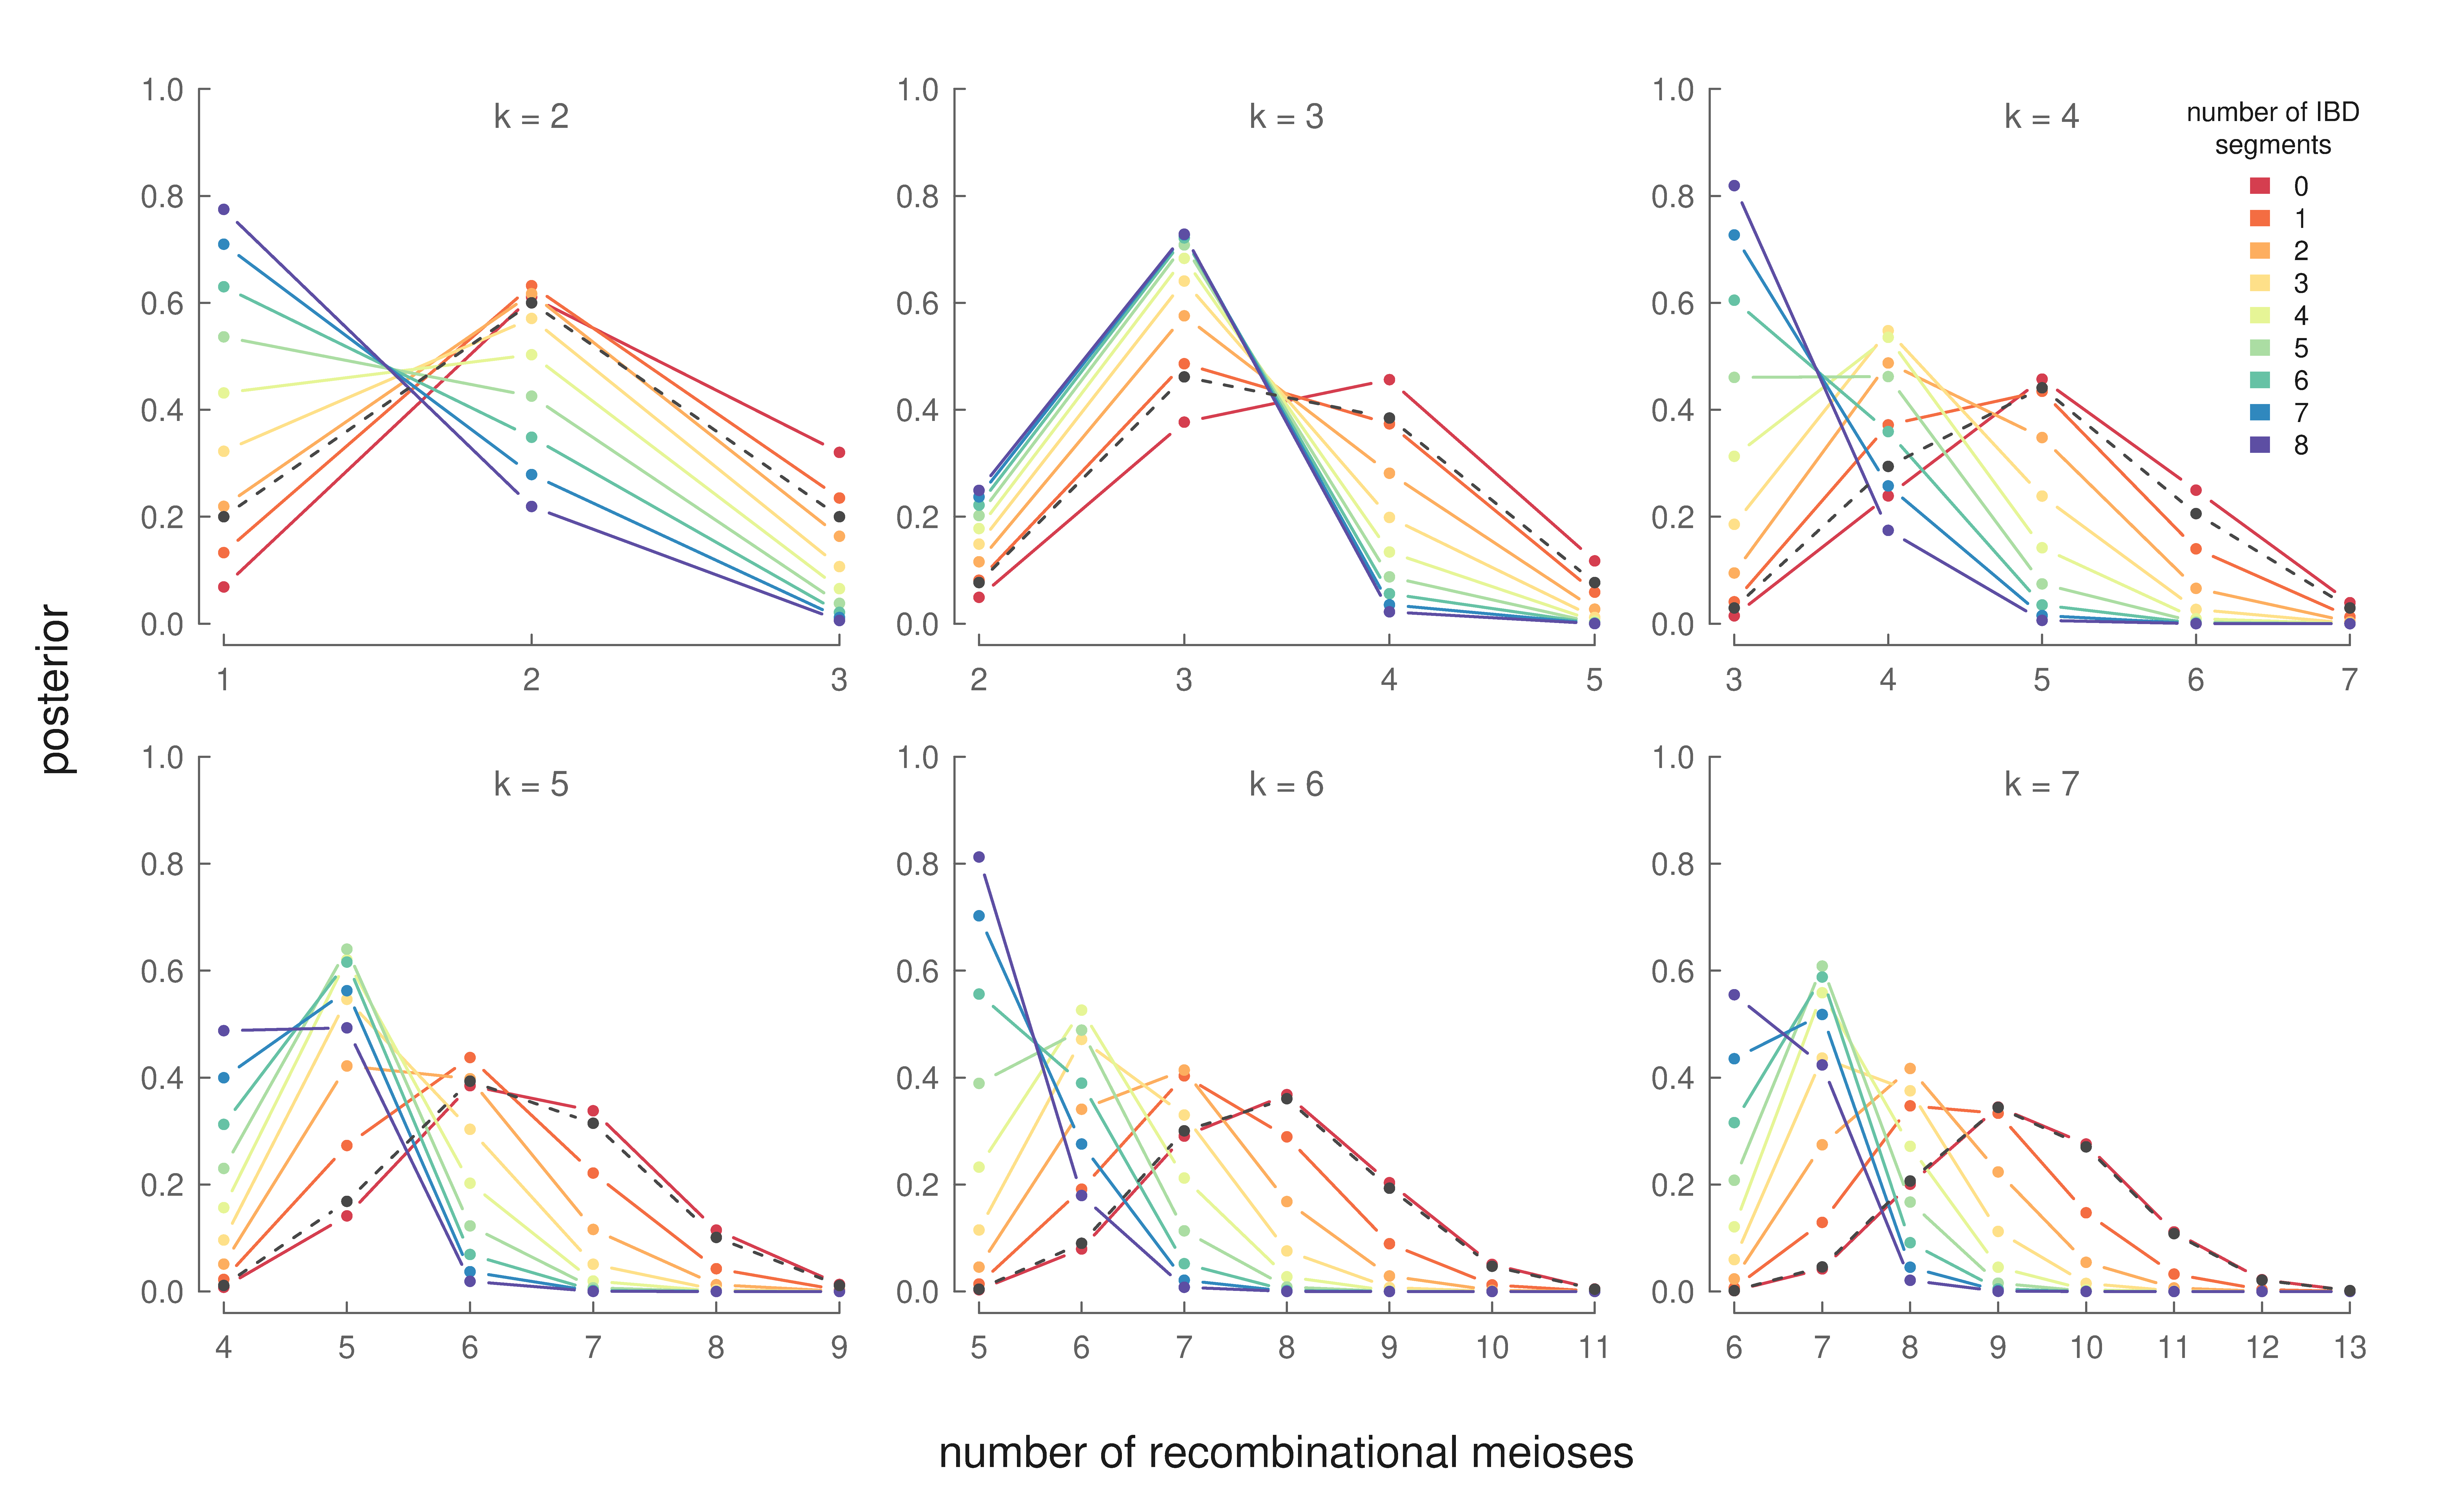
\includegraphics[width=\textwidth]{images/rm-posterior}

  \caption{Posterior probability distribution $P(R = r | N = n, k)$ for
different generations (each panel), and the observed number of IBD segments
(each colored line). The prior distribution of recombinational meioses given
$k$ is indicated by a black dashed line.}

  \label{fig:inference}

\end{figure}

In Figure \ref{fig:inference}, we show the posterior distributions over the
number of recombinational meioses, given an observed number of IBD segments
between two females known to be X half-cousins. Again, these posterior
distributions condition on knowing how many generations have occurred since the
shared ancestor, $k$.  With an increasing number of generations to the shared
ancestor, fewer segments survive to be IBD between the present-day cousins.
Consequently, observing IBD segments increases the likelihood of fewer females
(and thus fewer recombinational meioses) between the cousins. For example, for
$k=6$, observing (the admittedly unlikely) six or more IBD segments leads to a
posterior mode over the fewest possible number of females in the genealogical
chain ($\lfloor (2k-1)/2 \rfloor = 5$; Figure \ref{fig:inference}).  Similarly,
observing between three and five segments places the posterior mode over six
females in the genealogical chain. For $k>4$, seeing zero segments provides
little information over the prior about the relationship between the cousins,
as sharing zero segments is the norm.


\section{Discussion}

Detecting and inferring the nature of recent ancestry is important to a range
of applications and the nature of such relationships are often of inherent
interest.  As the sample sizes of population genomic data sets increase, so
will the probability of sampling individuals that share recent ancestry. In
particular, the very large data sets being developed in human genetics will
necessitate taking a genealogical view of recent relatedness.  Our methods
extend existing methods for the autosomes by accounting for the special
inheritance pattern of the X. Specifically, recent ancestry on the X differs
from the autosomes since males only inherit an X from their mothers, and
fathers pass an unrecombined (ignoring the PAR) X to their daughters.
Consequently, the number of recombinational meioses, which determine the length
and number of IBD segments, varies across the X genealogy. Since in most cases
the number of females between two individuals in a genealogical chain is often
unknown, we derive a distribution for recombinational meioses (equation
\eqref{eq:recomb-pmf}).

We derive distributions for the length and number of IBD X segments by
marginalizing over the unknown number of recombinational meioses that can occur
between two individuals connected through a genealogical chain. In both cases,
we condition on knowing $k$ (the generations back to a shared ancestor) which
can be inferred from the autosomes \citep{huff2011maximum}. Our models for IBD
segment number and length use a Poisson-Binomial approximation to the
recombination process, which match simulation results closely.

Our results here not only allow X IBD segments to be used to model recent
ancestry, but are in fact more informative about which genealogical ancestors
individuals share than autosomal data alone. This additional information occurs
through two avenues. First, sharing IBD segments on the X immediately reduces
the potential genealogical ancestors two individuals share, since one's X
ancestors are only a fraction of their possible genealogical ancestors (i.e.
$\mathcal{F}_{k+2}/2^{k}$ in the case of a present-day female). Second, the
varying number of females in an X genealogy across lineages combined with the
fact that recombinational meioses only occur in females to some extent leave a
lineage-specific signature of ancestry.

Unfortunately, the X chromosome is short, such that the chance of any signal of
recent ancestry on the X decays rather quickly. However, growing sample sizes
will increase both the detection of the pairwise relatedness and cases of
relatedness between multiple individuals. In these large data sets, overlapping
pairwise relationships (e.g. a present-day individual that shares X segments
with two distinct other individuals) could be quite informative about the
particular ancestors that individuals share. 

Our results should also be of use in understanding patterns of admixture on the
X chromosome. In particular our results about the posterior information from
the number and length of X segments shared with a genealogical ancestor can
help us understand what can be learned from the presence (or absence) of
particular segments of particular ancestry on the X chromosome. While this
information for an individual decays somewhat quickly after a small number of
generations, models of X chromosome segment ancestry will be useful at a
population-level for understanding sex-biased admixture
\citep{bryc2010genome,Goldberg:2015ja,Shringarpure039347}.

\section{Acknowledgements}

We wish to thank Nancy Chen, Jeremy Berg, Kristin Lee, and the rest of the Coop
lab for helpful discussions and feedback on earlier drafts. We also thank Amy
Williams and the Statistical and Computational Genetics Reading Group at
Cornell for very helpful feedback on the BioRxiv preprint version. Finally, we
thank Noah Rosenberg and two anonymous reviewers for their feedback.
%
This research was supported by an NSF Graduate Research Fellowship grant
awarded to VB (1148897), and National Institute of General Medical
Sciences of the National Institutes of Health under award numbers NIH
RO1GM83098 and RO1GM107374 to GC.

\printbibliography
\nocite{kram2015}
\nocite{dplyr}
\nocite{ggplot2}
\nocite{R}
\nocite{Rossum:1995:PRM:869369}
\nocite{C}
\nocite{colorspace}
\nocite{purrr}
\nocite{tidyr}

\newpage
\appendix

\section{Convergence of the Thinned Poisson Process to Poisson-Binomial Model}
\label{ap:pois-thin}

We compared the Poisson thinning approximation and the Poisson-Binomial models.
One can show using the law of total expectation that the Poisson-Binomial and
Poisson model have the same expected value:

\begin{align}
  \E[N] &= \sum_{b=0}^\infty \E[N | B = b]P(B = b)\\
  \E[N] &= 1/2^d \left( \sum_{b=0}^\infty b \text{Pois}(B = b) + c \sum_{b=0}^\infty \text{Pois}(B = b) \right) \\
  \E[N] &= \frac{1}{2^d} (\nu d + c)
\end{align}
%
This is the same expected value as the thinned Poisson process with rate $(\nu
d + c)/2^d$. However, the Poisson thinning and Poisson-Binomial models differ
in their variance. Using Eve's law, we can show the Poisson-Binomial model has
variance
%
\begin{align}
  \label{eq:n-variance}
  \V[N] &= \E_B[\V[N | B]] + \V_B[\E[N|B]]\\
  \V[N] &= \frac{dv + 1}{2^d} - \frac{1}{2^{2d}}
\end{align}
%
This differs from the thinned Poisson process variance by the term
$\nicefrac{1}{2^{2d}}$, which grows smaller with increasing $d$. Finally, we
numerically show these two distributions (here, we label the two distributions
for $k$ generations $\mu_k(x)$ and $\nu_k(x)$, where $x$ is the number of
segments) converge quickly in total variational distance ($d_{TV}(\mu_k, \nu_k) =
\nicefrac{1}{2}\sum_{n = 0}^\infty | \mu_k(n) - \nu_k(n) |$) as $k$ increases,
in Figure \ref{fig:total-var-dist}.

\begin{figure}[!ht]
  \centering
  
\includegraphics[width=0.7\textwidth]{images/total-var-dist}

  \caption{The total variation distance between the Poisson thinning and the
  Poisson-Binomial model for IBD segment number for X segments (yellow) and the
autosomal segments (blue).}

\label{fig:total-var-dist}
\end{figure}

\section{Generating Function for Recombinational Meioses}
\label{ap:generating-function}

We also develop a generating function $g(x, k)$ that encodes the number of
recombinational meioses in the $k^{\text{th}}$ generation as the coefficient
for the term $x^k$. This generating function can also be used in approximations
and finding moments of the distribution $p_k(r)$.

\begin{lemma}
  An expansion of the generating function below encodes the number of lineages
  with $r$ females in a genealogical chain $k$ generations long ($n_{k,r}$) as
  the coefficient of the term $x^{k}$

  \begin{align}
    g(x, k) = \frac{1}{2^{k+1}\sqrt{x} \sqrt{x+4}}
    \left[x
    \left(\left(R^+\right)^k - \left(R^-\right)^k\right) + \sqrt{x} \sqrt{x+4}
    \left(\left(R^-\right)^k + \left(R^+\right)^k\right)
    -2 \left(R^-\right)^k+2 \left(R^+\right)^k\right]
  \end{align}

  \text{where}

\begin{align}
    R^- &= x-\sqrt{x} \sqrt{x+4}\\
    R^+ &= x+\sqrt{x} \sqrt{x+4}
\end{align}

\end{lemma}

\begin{proof}

 We begin by stating some recurrences that occur from the inheritance pattern of
 X ancestry:

\begin{enumerate}
  \item $ n_{k,r} = m_{k,r} + f_{k,r} $
  \item $ m_{k,r} = f_{k-1,r} $
  \item $ f_{k,r} = f_{k-1, r-1} + m_{k-1,r-1} $
\end{enumerate}

Starting from (1):

\begin{align} 
   n_{k,r} &= m_{k,r} + f_{k,r} \\
   n_{k,r} &= f_{k-1,r} + f_{k,r} \\
   n_{k,r} &= f_{k-1,r} + f_{k-1, r-1} + m_{k-1,r-1} \\
   n_{k,r} &= f_{k-1,r} + n_{k-1, r-1} \\
   n_{k,r} &= f_{k-2, r-1} + m_{k-2,r-1} + n_{k-1, r-1} \\
\end{align}

finally, substituting (1) again gives us the desired recurrence relation
for $n_{k,r}$:

\begin{align} \label{eq:recur-01}
   n_{k,r} &= n_{k-2, r-1} + n_{k-1, r-1}
\end{align}

We can now use generating functions \citep{wilf2013generatingfunctionology} to
tackle this recurrence. Define:

\begin{equation}
  A_k(x) = \sum_{r \ge 0} n_{k,r} x^r
\end{equation}

then, multiply both sides of \eqref{eq:recur-01} by $x^r$ and sum over $r$. On
the right hand side:

\begin{align}
  &= \sum_{r \ge 0} n_{k-2, r-1} x^r + \sum_{r \ge 0} n_{k-1, r-1} x^r
\end{align}

 Note that $n_{k,r} = 0$ if $r < 0$. Multiplying and dividing the second term by
 $x$ yields:

 \begin{align}
   x(n_{k-1, 0} x + n_{k-1, 1} x^2 + n_{k-1, 2} x^3 + \ldots)/x = x A_{k-1}(x) 
 \end{align}

 An identical derivation works for the first term. We find:

 \begin{equation} \label{eq:rec-gen}
   A_k(x) = xA_{k-1}(x) + xA_{k-2}(x)
 \end{equation}

This generating function is in the form of another recurrence. We can solve
this recurrence (i.e. with Mathematica) with the initial conditions below
(which can be derived from \eqref{eq:recur-01} and its initial conditions)
%
\begin{enumerate}
  \item $ A_0(x) = 1 $
  \item $ A_1(x) = 1 + x $
\end{enumerate}
%
to find a solution with these initial conditions, giving us our desired
generating function $g(x,k)$.

\end{proof}

We can see that our generating function works via an expansion and verify
the coefficients match known numbers of recombinational meioses for some $k$.
For example, let's expand $g(x, k)$ at $k=5$:

\begin{equation*}
  x^2 + 6x^3 + 5x^4 + x^5
\end{equation*}
%
which matches the $n_{k,r}$ values found via computational calculation.

\section{Half-Cousins IBD Length Distribution Simulation Results}

Figure \ref{fig:half-cousin-x-length} show the concordance between our cousin
IBD segment length analytic distributions and the binned average (1.98cM bin
intervals) of 5,000 simulations.

\begin{figure}[!ht]
  \centering
  
\includegraphics[width=\textwidth]{images/x-halfcousins-blocklens}

  \caption{The analytic distributions of IBD segment length (blue lines)
  between two-present-day female half-cousins with a shared ancestor in the
$k^\text{th}$ generation (each panel), and the binned average 5,000
simulations (gray points).}

\label{fig:half-cousin-x-length}

\end{figure}

\section{An Approximation of X Pedigree Collapse}
\label{ap:ped-collapse}

Since our models of recent X ancestry omit the possibility of pedigree
collapse, it is worthwhile to see when this assumption breaks down. To see how
pedigree collapse becomes an increasing problem further generations back, we
look at the probability that all of a single individual's $\mathcal{F}_{k+2}$ X
ancestors, when sampled from a population of $N$ individuals with replacement,
are distinct. We treat generations as discrete and non-overlapping, and look at
the probability that all $\mathcal{F}_{k+2}$ are distinct individuals as a
function of how many generations we go back. This problem is similar to the
celebrated birthday problem, but with two rooms of participants: one room of
females and another of males. Assuming random mating, each generation, one's X
ancestors must be randomly selected with replacement from a population of $N$
individuals. For all ancestors to be distinct, all $\mathcal{F}_{k}$ male
ancestors selected from a pool of $N/2$ and $\mathcal{F}_{k+1}$ female
ancestors selected from a pool of $N/2$ must be unique:

\begin{align}
  P(\text{X ancestors all distinct}) &= P(\text{male X ancestors unique}) P(\text{female X ancestors unique})\\
                                     &= \prod_{i=1}^{\mathcal{F}_{k}} \left(1-\frac{2i}{N}\right)\prod_{j=1}^{\mathcal{F}_{k+1}} \left(1-\frac{2j}{N}\right)
\end{align}

This probability as a function of $k$ is plotted in Figure
\ref{fig:ped-collapse}. For X ancestors, the probability that at least two
individuals are non-distinct only becomes a significant problem after around 12
generations. Note that this is a very conservative account of how pedigree
collapse could affect our calculations; even if two ancestors were to be
non-distinct, this is unlikely to affect our calculations greatly. For pedigree
collapse to affect our IBD segment models, an individual has to both be a
genealogical ancestor \emph{and} a genetic ancestor of the present-day
individual; pedigree collapse has no genetic affect if non-distinct individuals
are not genetic ancestors.

\begin{figure}[!ht]
  \centering
  
\includegraphics[width=0.6\textwidth]{images/ped-collapse}
  \caption{The probability that all genealogical and X ancestors are distinct in a population of $N=100,000$.}
  \label{fig:ped-collapse}
\end{figure}

For other pedigree collapse related quantities (e.g., what's the average number
of distinct ancestors $k$ generations back), see
\textcite{wachter2013statistical} approximations which use Feller's
(\citeyear{feller1950introduction}) occupancy models.


\end{document}
